\chapter{二维多铁材料}

\section{二维材料}

二维材料有很多种一般并不存在于自然界中,绝大部分二维材料是人工合成或制造的,自从石墨烯被发现之后,二维材料以其多种多样的性质受到人们的广泛关注。以二维材料为代表低维材料在一个或多个维度上空间尺度与微观粒子尺度相近似,支配微观世界的量子力学等微观规则与性质会在宏观尺度上表现出来,研究低维材料对解决基础理论或实际应用上面重大问题有很大帮助。\cite{novoselov2004electric}随着对铁磁、铁电和多铁材料的进一步研究,对新物理、新材料的研究使研究对象由高维(三维)向低维扩展。

多年以来,对常规的三维多铁材料的研究有很多进展,但至今没有一种广泛应用的在室温下稳定的多铁材料进入应用领域。另一方面,由于二维材料在一个方向上有着与微观粒子相同的尺度,二维材料常常有着与常见的三维材料截然不同的性质与现象,二维材料可能在自发极化强度、电磁耦合强度等各种基本性质上与三维材料有着显著差异。对多铁性来说,材料的降维会是对称性元素减少,有利于铁电性、铁磁性等对称性破缺等性质的产生。另外二维材料巨大的比表面积使其更容易受到外在环境变化的影响,采用外加电磁场、进行原子、分子、离子吸附掺杂等方法进而改良物理性质变得更加容易。然而,受制于二维材料不稳定的先天缺陷,低成本、稳定的、可实用二维材料的寻找、制备、应用的过程会比常见的三维材料更加困难。

\section{二维材料的磁性质}
二维材料不仅拥有很多新的电子学性质,还拥有很多新奇的磁学性质。同非二维材料一样,二维材料的磁性是来源于电子轨道之中的未配对电子。由泡利不相容原理以及洪特规则可得,最先填充一个电子壳层的若干电子自旋方向倾向于相同,这些电子将优先占据能量较低多数多数自旋态而使局域原子显出磁矩。局域磁矩按照一定规律排列组合,即可在宏观尺度上表现出磁性。二维磁性材料像三维磁性材料一样,也可以分为铁磁性、亚铁磁性、反铁磁性、顺磁性、抗磁性。铁磁性二维材料具有自发极化磁矩,在外场作用下可以实现磁矩方向的翻转,在外场撤出后仍然保留比较大的剩余磁化强度,有着广泛的应用前景与研究价值。

目前发现的二维材料大多不具备铁磁性,二维材料之中产生铁磁性的重要一点是在二维材料内部产生未配对电子,进一步使二维材料的电子态密度产生自旋劈裂,即不同自旋方向的电子态密度出现不对称。从二维材料的能带结构上面看来,二维铁磁材料可以分为三种:铁磁半导体、铁磁导体、铁磁金属。铁磁半导体在发生自旋能级分裂时没有被费米面穿过,与半导体一样存在带隙。铁磁导体中发生自旋分裂的两种自旋方向能级被费米面穿过,没有带隙。铁磁半金属有一个自旋方向的态密度被费米面穿过,没有带隙,另一个自旋方向没有被穿过,存在带隙保持着绝缘体或者半导体的性质,对一个自旋方向的电子来说是导体,对另一种自旋方向的电子来说是绝缘体,这种半金属半绝缘体的性质可以用来选择性过滤某种自旋方向的电子。为增强铁磁性,通常在二维材料之中,一般采取载流子掺杂的方式,提高费米面附近电子密度,进而引发电子自旋分裂产生铁磁性。

\begin{figure}[h]
    \centering
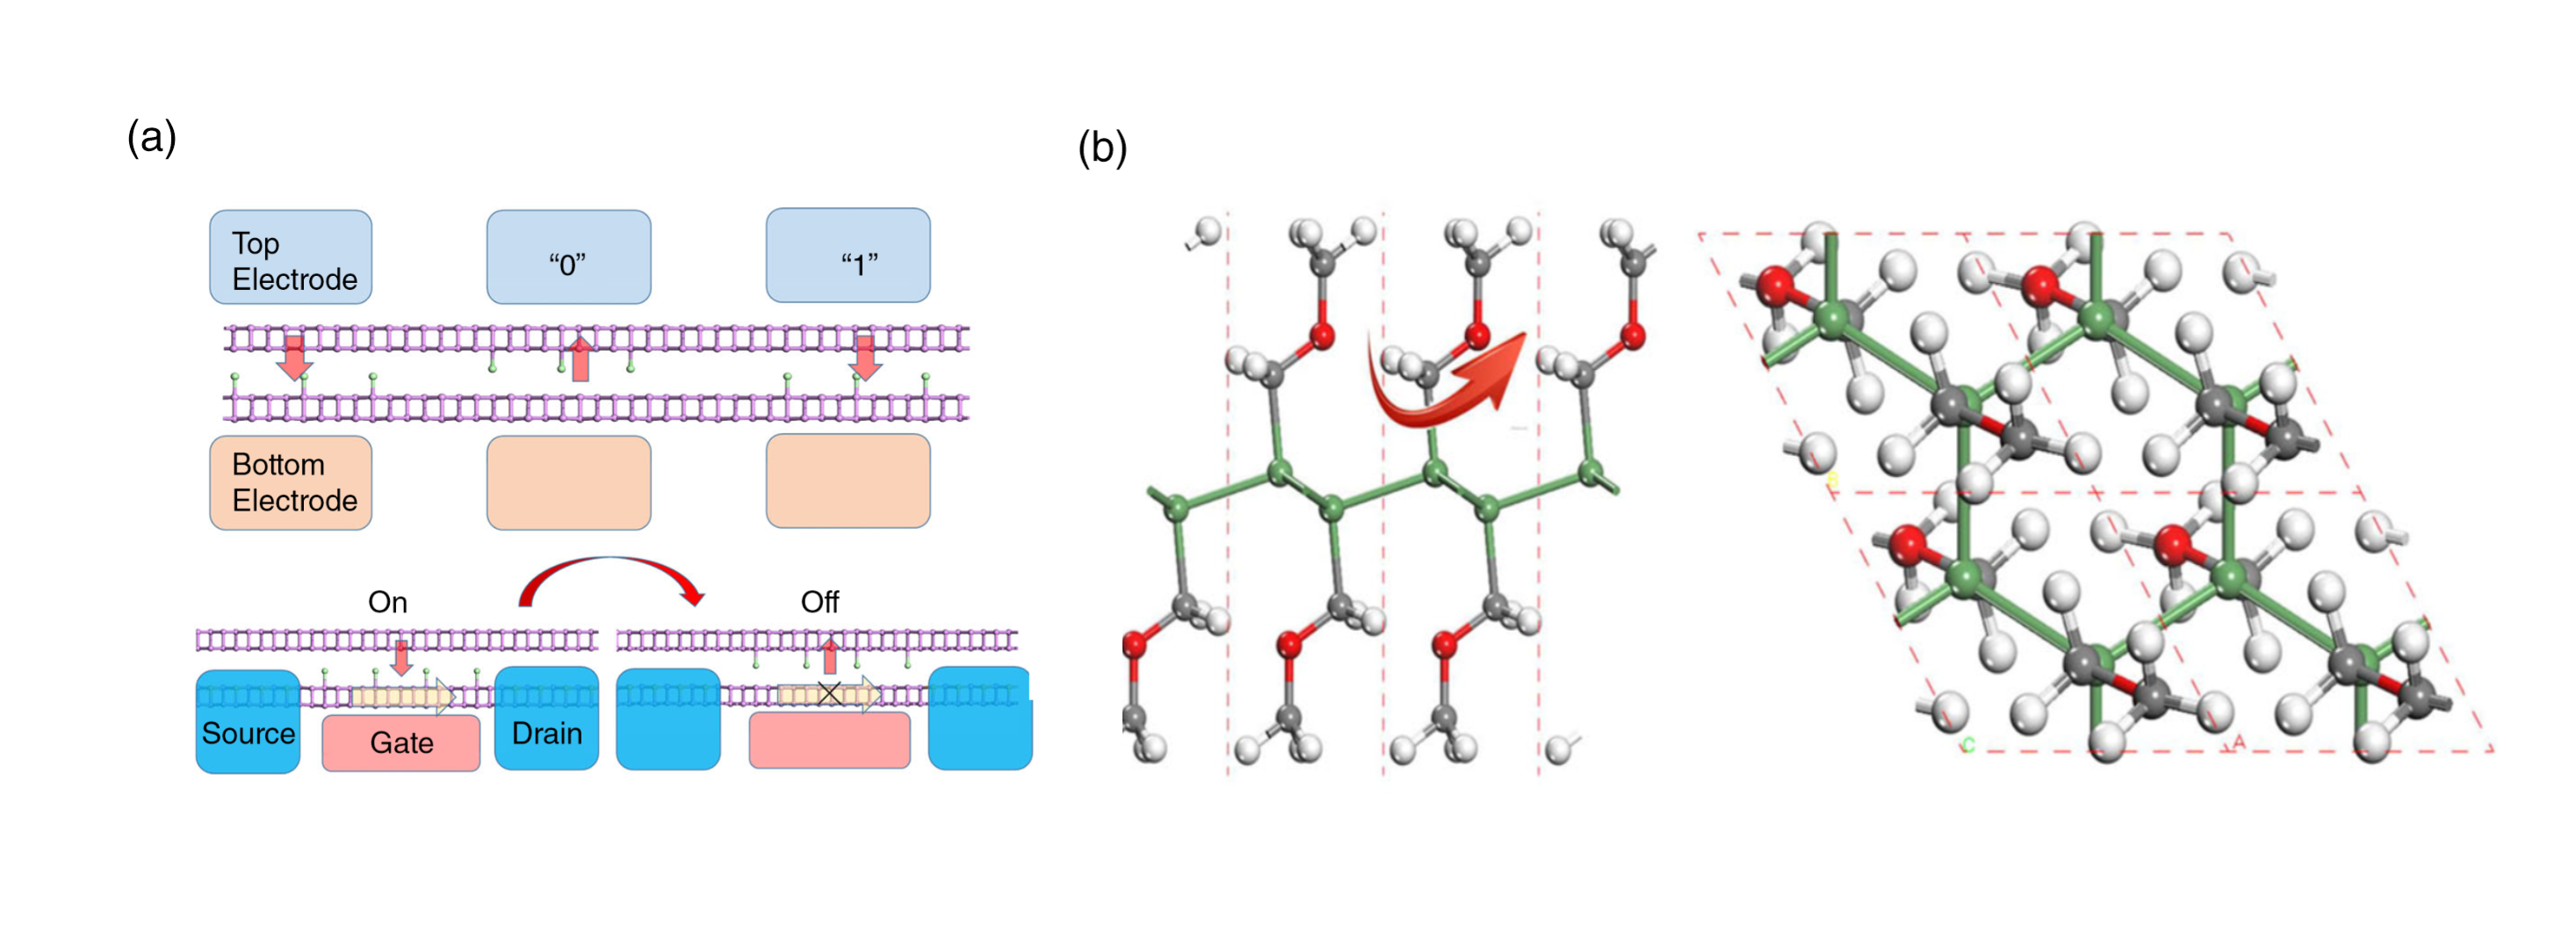
\includegraphics[width=0.8\textwidth]{./pic/015.png}
\caption{(a)卤素原子在磷烯双层之间的迁移形成垂直二维平面的电极化,通过外加电场使卤素原子在两层间的迁移实现电极化的反转,可以用来制作磁读电写存储器与多铁场效应管 \ (b)添加$CH_{2}OCH_{3}-$后的锗烯层,通过添加后的极性官能团在平面内的旋转实现电极化方向的转换}

\label{dog015}
\end{figure}

\section{二维材料的铁电性}

与三维材料一样,铁电性是由自发极化的电偶极矩形成的,微观层面的正负电荷中心不重合产生的电偶极矩,按照一定的规律组合叠加起来,最终形成宏观的电偶极矩。目前发现的具有铁电性的二维材料比较少,主要来源于中心对称缺失的二维晶体结构。

\begin{table}[!htbp]
    \caption{常见的二维铁电材料}
    \label{tab:dog}
    \resizebox{\textwidth}{!}{
    \begin{tabular}{lllllc}
        \toprule
        
        材料 & 极化强度(pC/m) & 电极化方向 & FE switch barrier(meV/f.u.) & 转变温度(K) &参考资料 \\
        \midrule
        1T-$MoS_{2}$ & 0.28 $μC/cm^{2}$ & 垂直平面 & 未见报道 & 未见报道 & \cite{shirodkar2014emergence} \\
        Group IV binary AB, Group III–V binary AB & 0.88–4.22, 7.82–11.45O&垂直平面&160–390, 50–300&未见报道&\cite{di2015emergence}\\
        SnS, SnSe, GeS, GeSe&151–506&面内&3.76–580.77&326–6400&   \cite{fei2016ferroelectricity}\\
        $\beta -GeSe$&160&面内&5.83&200&\cite{guan2018tunable}\\

        As, Sb, Bi&46–151&面内&5.83–183.6&463–680&\cite{xiao2018elemental}\\
        SnTe&未见报道&面内&未见报道&270&\cite{chang2016discovery}\\
        GeTe&32.8$μC/cm^{2}$&面内&37.4&570&\cite{wan2017promising}\\
        $\alpha -In_{2}Se_{3}$&2.36e Å, 0.11e Å&面内,垂直平面&57T&室温&\cite{ding2017prediction}\cite{zhou2017out}\cite{cui2018intercorrelated}\\
        $\beta -In2Se3$&未见报道&面内&未见报道&473&\cite{zheng2018room}\\
        $WTe_{2}$&~0.16&垂直平面&未见报道&350&\cite{fei2018ferroelectric}\\
        $CuInP_{2}S_{6}$&未见报道&垂直平面&未见报道&320&\cite{liu2016room}\\
        $AgBiP_{2}Se_{6}$&1.2&垂直平面&6.2&超过室温& \cite{xu2017monolayer}\\
        $CuInP_{2}Se_{6}$&0.322$μC/cm^{2}$&垂直平面&80&150&\cite{song2017off}\\
        Graphene-OH&6.6$μC/cm^{2}$&面内&未见报道&700&\cite{kan2013high}\\
        Ge, Si, SnSb, $MoS_{2}$−SAM&31–117&面内&~90 per ligand&超过350&\cite{wu2016ferroelectricity}\\
        Sc2CO2&176, 1.60μC/cm2&面内,垂直平面&520&超过室温&   \cite{chandrasekaran2017ferroelectricity}\\

        \bottomrule
    \end{tabular}}
\end{table}


\subsection{固有极化的二维铁电材料}

通常来说,铁电材料在居里温度以下会产生自发极化,外加电场很容易影响这种自发极化的大小与方向。二维材料产生自发极化,必然有着一个使系统对称性降低极化方向,一个与众不同的特殊方向方向。到目前为止,有一部分二维铁电材料被发现。这些材料的组成元素具有多样性,自发极化的方向有平面内的和垂直于二维平面的,其性质也各不相同。

\begin{figure}[h]
    \centering
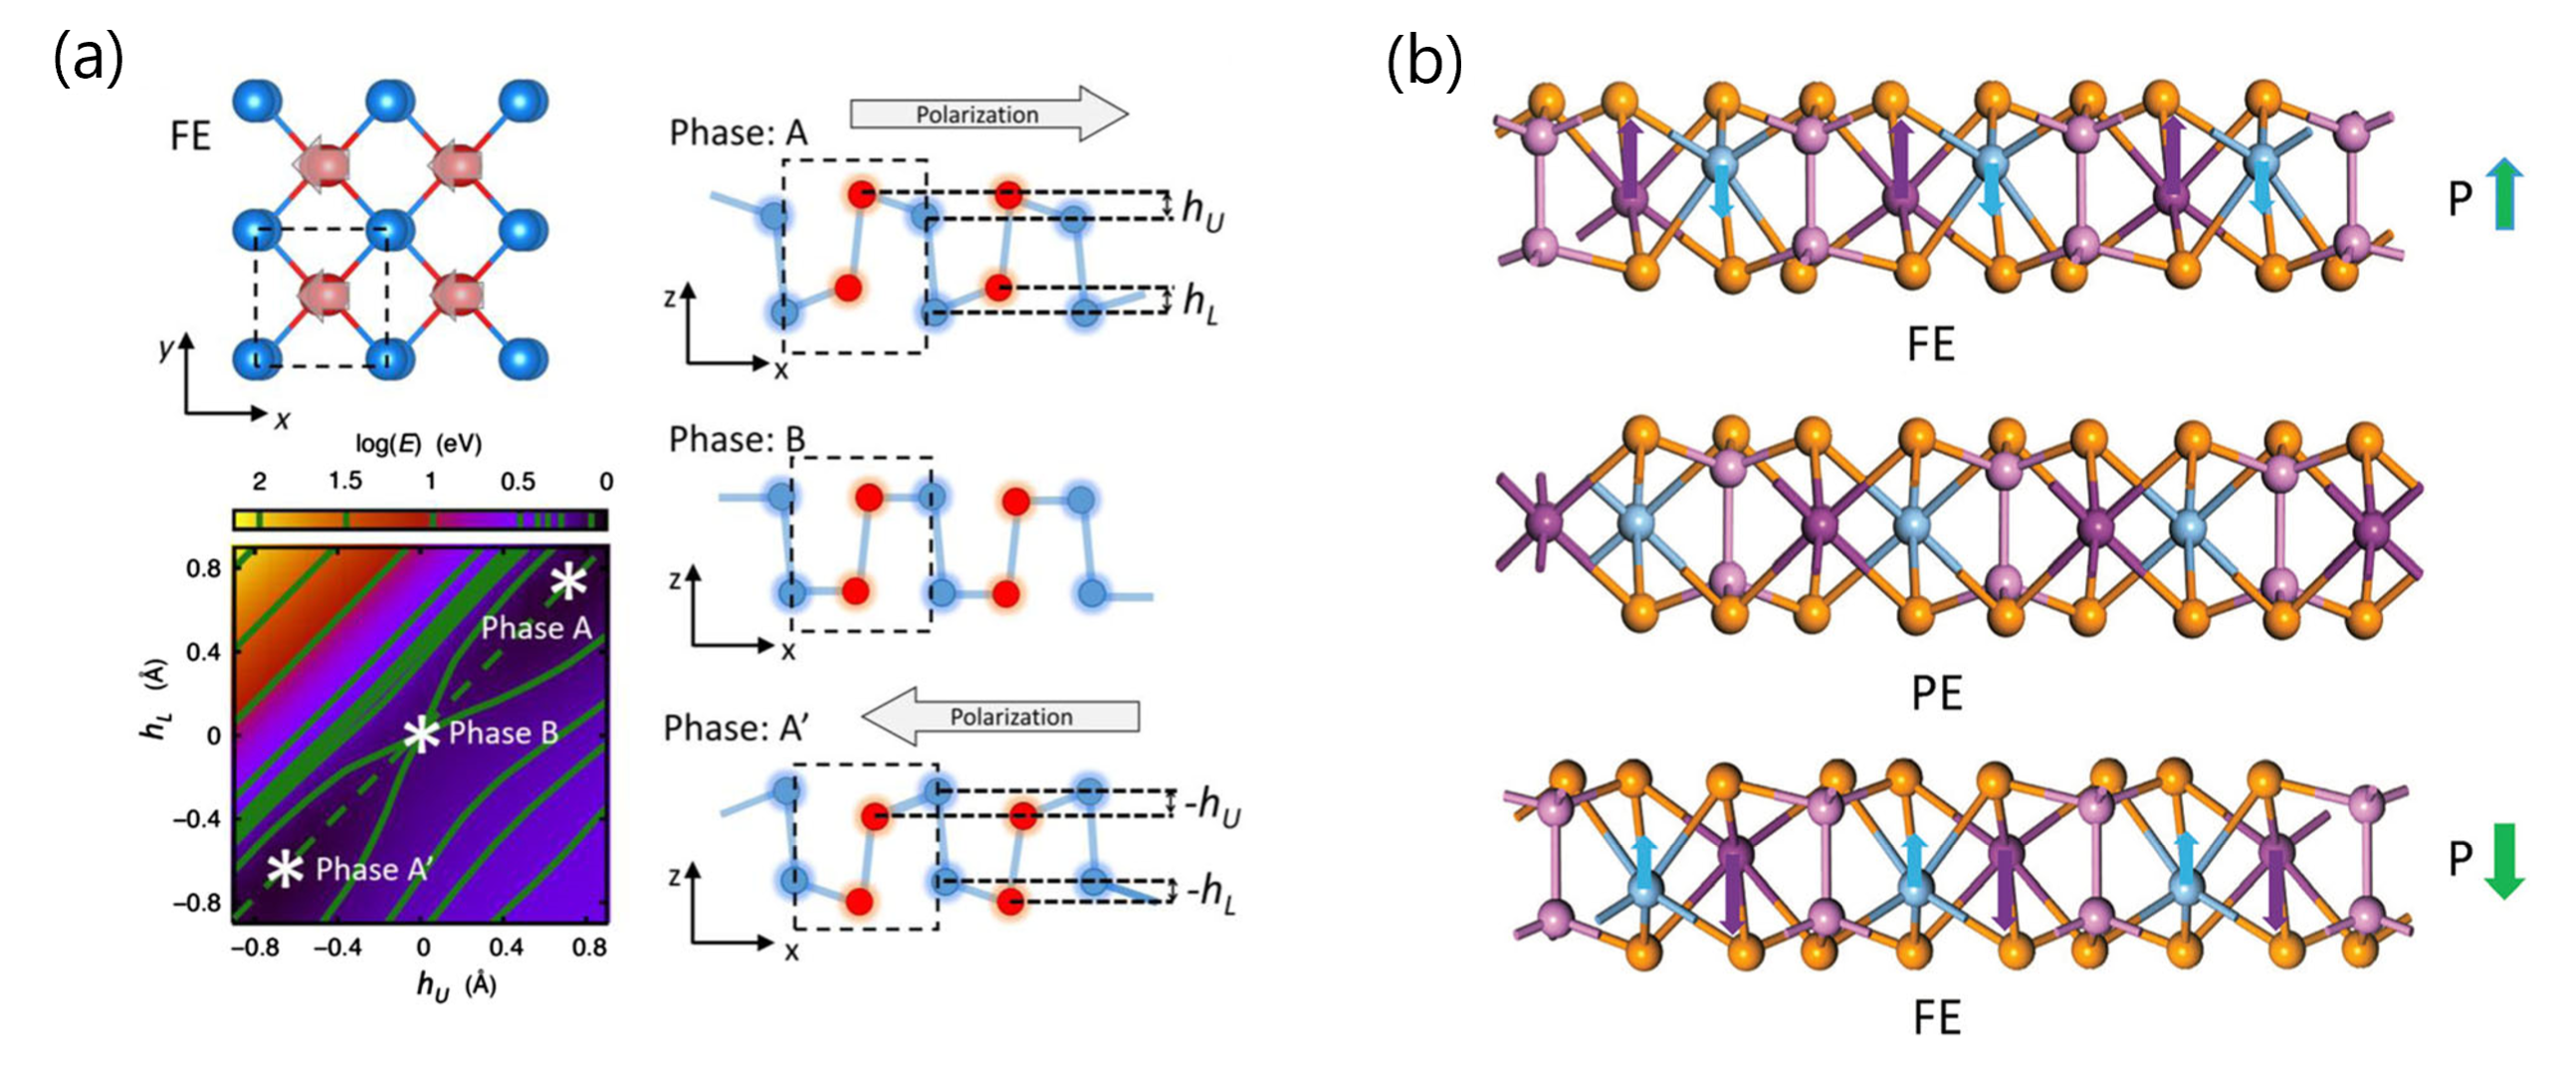
\includegraphics[width=0.8\textwidth]{./pic/016.png}
\caption{(a)第五主族元素形成的二维铁电材料,晶格不同的畸变扭曲方式形成了三个相,其中两个不对称的铁电相,一个对称的没有电极化的相(b)复杂组分的二维铁电材料通过离子不同的位移形成电极化}

\label{dog016}
\end{figure}

$MoS_{2}$ 是一种在垂直二维平面产生极化的二维铁电材料,其单层结构的垂直极化大约可达$0.28μC/cm^{2}$。在第四主族元素或者第三到第五主族元素形成的二元二维膜中也发现过二维铁电材料,例如$SiGe\text{、}SiSn\text{、}GeSn\text{、}AlSb\text{、}GaP\text{、}GaAs\text{、}InP\text{、}InAs\text{、}InSb$等。以上这两种情况产生的主要是垂直二维平面的电极化。同样也存在面内自发电极化的二维材料。第四主族的硫族化合物MX((M = Ge, Sn; X = S,Se)是一种典型的二维面内极化铁电材料,这种材料的铁电性质与铁弹性有着较密切的关系。二维平面内部的压力产生的机械形变是导致其自发极化产生铁电性的重要原因,外电场对自发极化的正负电荷中心的作用同样会导致晶格结构产生畸变。其中GeSe的稳定性强,其电极化强度易受外力影响,是一种潜力巨大的二维铁电材料。单一元素构成的二维层状结构也可能存在铁电性,经过第一性原理计算,第五主族的As、Sb和Bi存在着稳定的面内铁电性,二维结构对sp3杂化的影响使部分原子出现位移磷烯结构产生扭曲。另一大类二维多铁材料是第三主族与第六主族的化合物,以$In_{3}Se_{2}$为典型代表的这类二维多铁材料有着面内和垂直于平面的自发极化,在具有这两种方向的电极化的同时,在室温下有较高的稳定性。

\begin{figure}[h]
    \centering
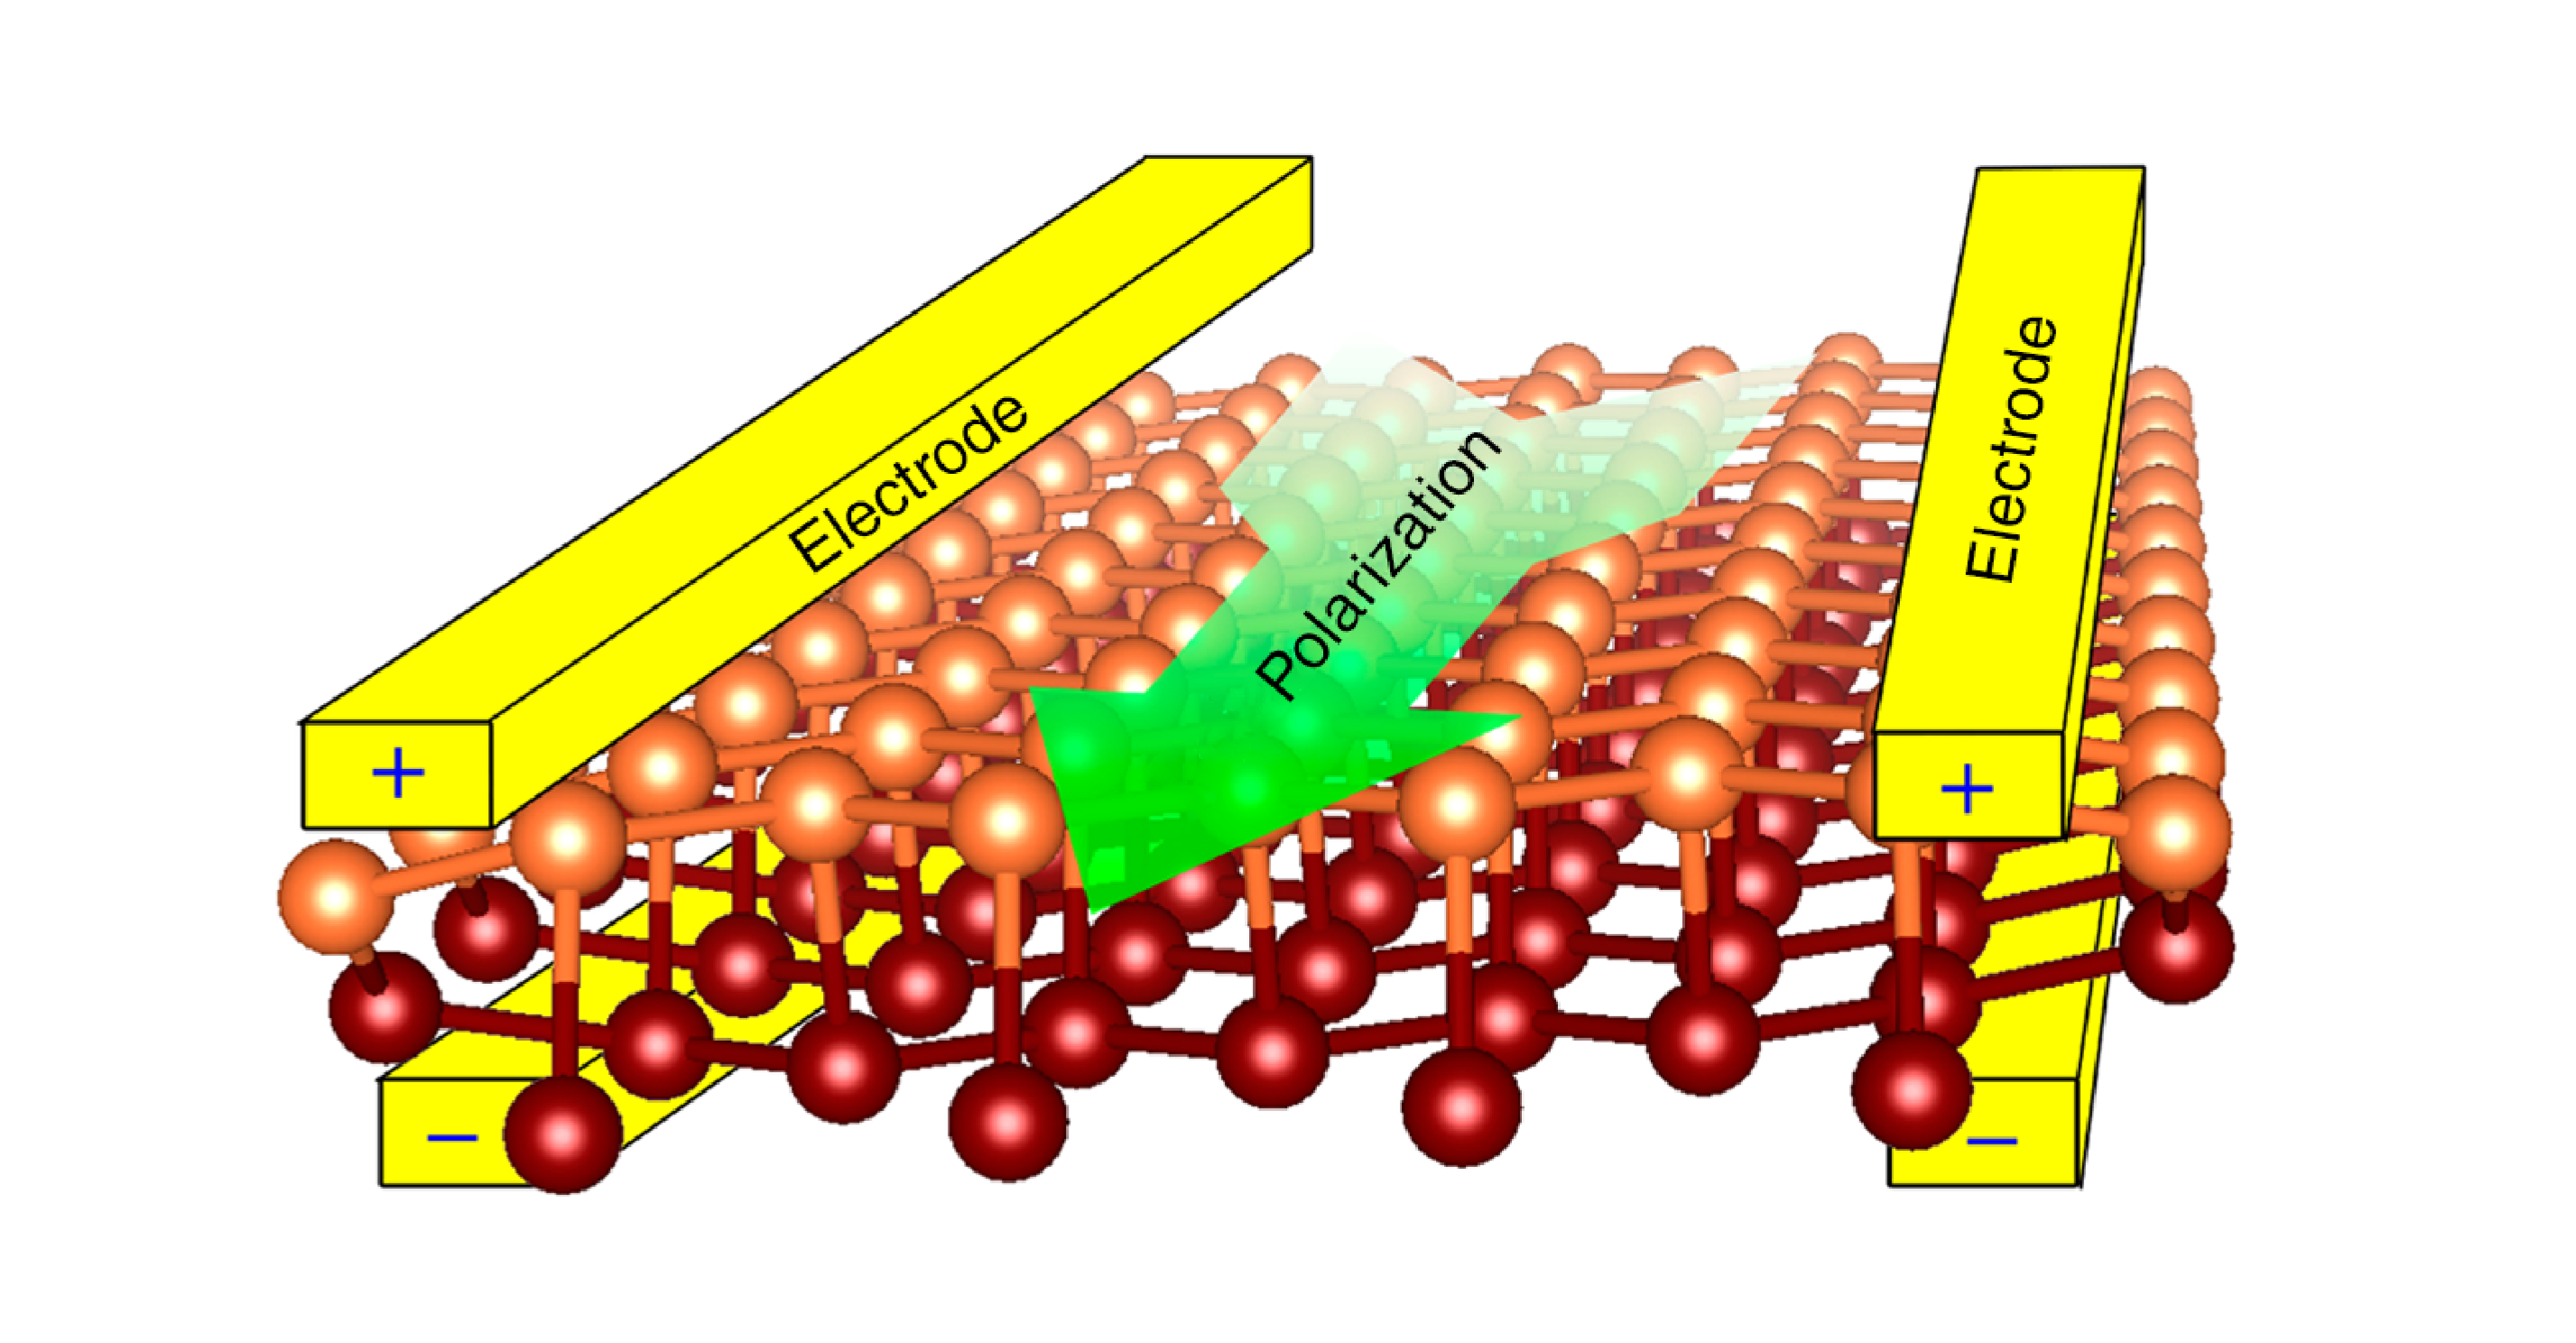
\includegraphics[width=0.8\textwidth]{./pic/013.png}
\caption{二维磷烯结构,垂直平面的外加电场导致平面内部产生电极化}

\label{dog013}
\end{figure}

通常认为,具有铁电性质的材料应该是绝缘体,导体中的自由电荷、载流子会在外加电场的影响下产生定向移动,进而会屏蔽掉外场对物质结构内部的作用,起到了电磁屏蔽的作用,阻碍外部电场对电极化方向的翻转作用。然而,在二维材料等低维材料中,由于几何因素等的限制,情况会有所不同。低维材料的若干个维度缺失会限制载流子对内部结构的电磁屏蔽作用,例如在二维材料中,面内部的粒子结构很难屏蔽垂直平面的电磁场对整个二维平面的影响,从而半导体甚至于导体都有可能出现铁电性。最近发现,两到三层拓扑半导体$WTe_{2}$电极化消失的温度在350K以上,经过第一性原理计算表明,将其置于两层石墨烯之间可进一步增强$WTe_{2}$二维层状结构在室温下的稳定性。

既然简单的只有一到两种元素组成的二维材料存在铁电性,更复杂的由多种元素组成的二维材料同样具有铁电性。过渡金属硫代磷酸酯(transition metal thiophosphate,TMTP)这类复杂的二维材料同样具有铁电性,这类复杂的二维材料的铁电性通常是由金属阳离子的位移与空间晶格扭曲引起的。$ AgBiP_{2}Se_{6}$对可见光有强吸收,可以作为光催化剂应用在水在光下分解等场合。

\subsection{诱导产生铁电性的二维材料}

除了二维材料本身带有的固有铁电性,一些二维材料可以被外围条件诱导产生铁电性。常见的诱导方式有吸附、应力和外场。二维材料具有巨大的表面积,十分容易吸附一些其余的原子分子离子。石墨烯吸附羟基官能团后面内会产生电极化,这与质子位移有关。一系列的二维材料例如硅烷、锗烷、$MoS_{2}$分子层等,吸附一些自组装官能团(OH,SH,CH3,CF3,NH2等)之后,会在面内产生电极化。外加吸附上去的分子很大可能会破坏了平面内的对称性,导致了特殊方向的出现。同样的,外加应力也会导致平面内部的对称性破缺,从而引发电极化,例如PbTe,适当的二维压缩会是其从正常相向铁磁相转化。对于磷烯纳米层,在垂直平面方向上施加电场会导致在面内出现电极化。

\begin{figure}[h]
    \centering
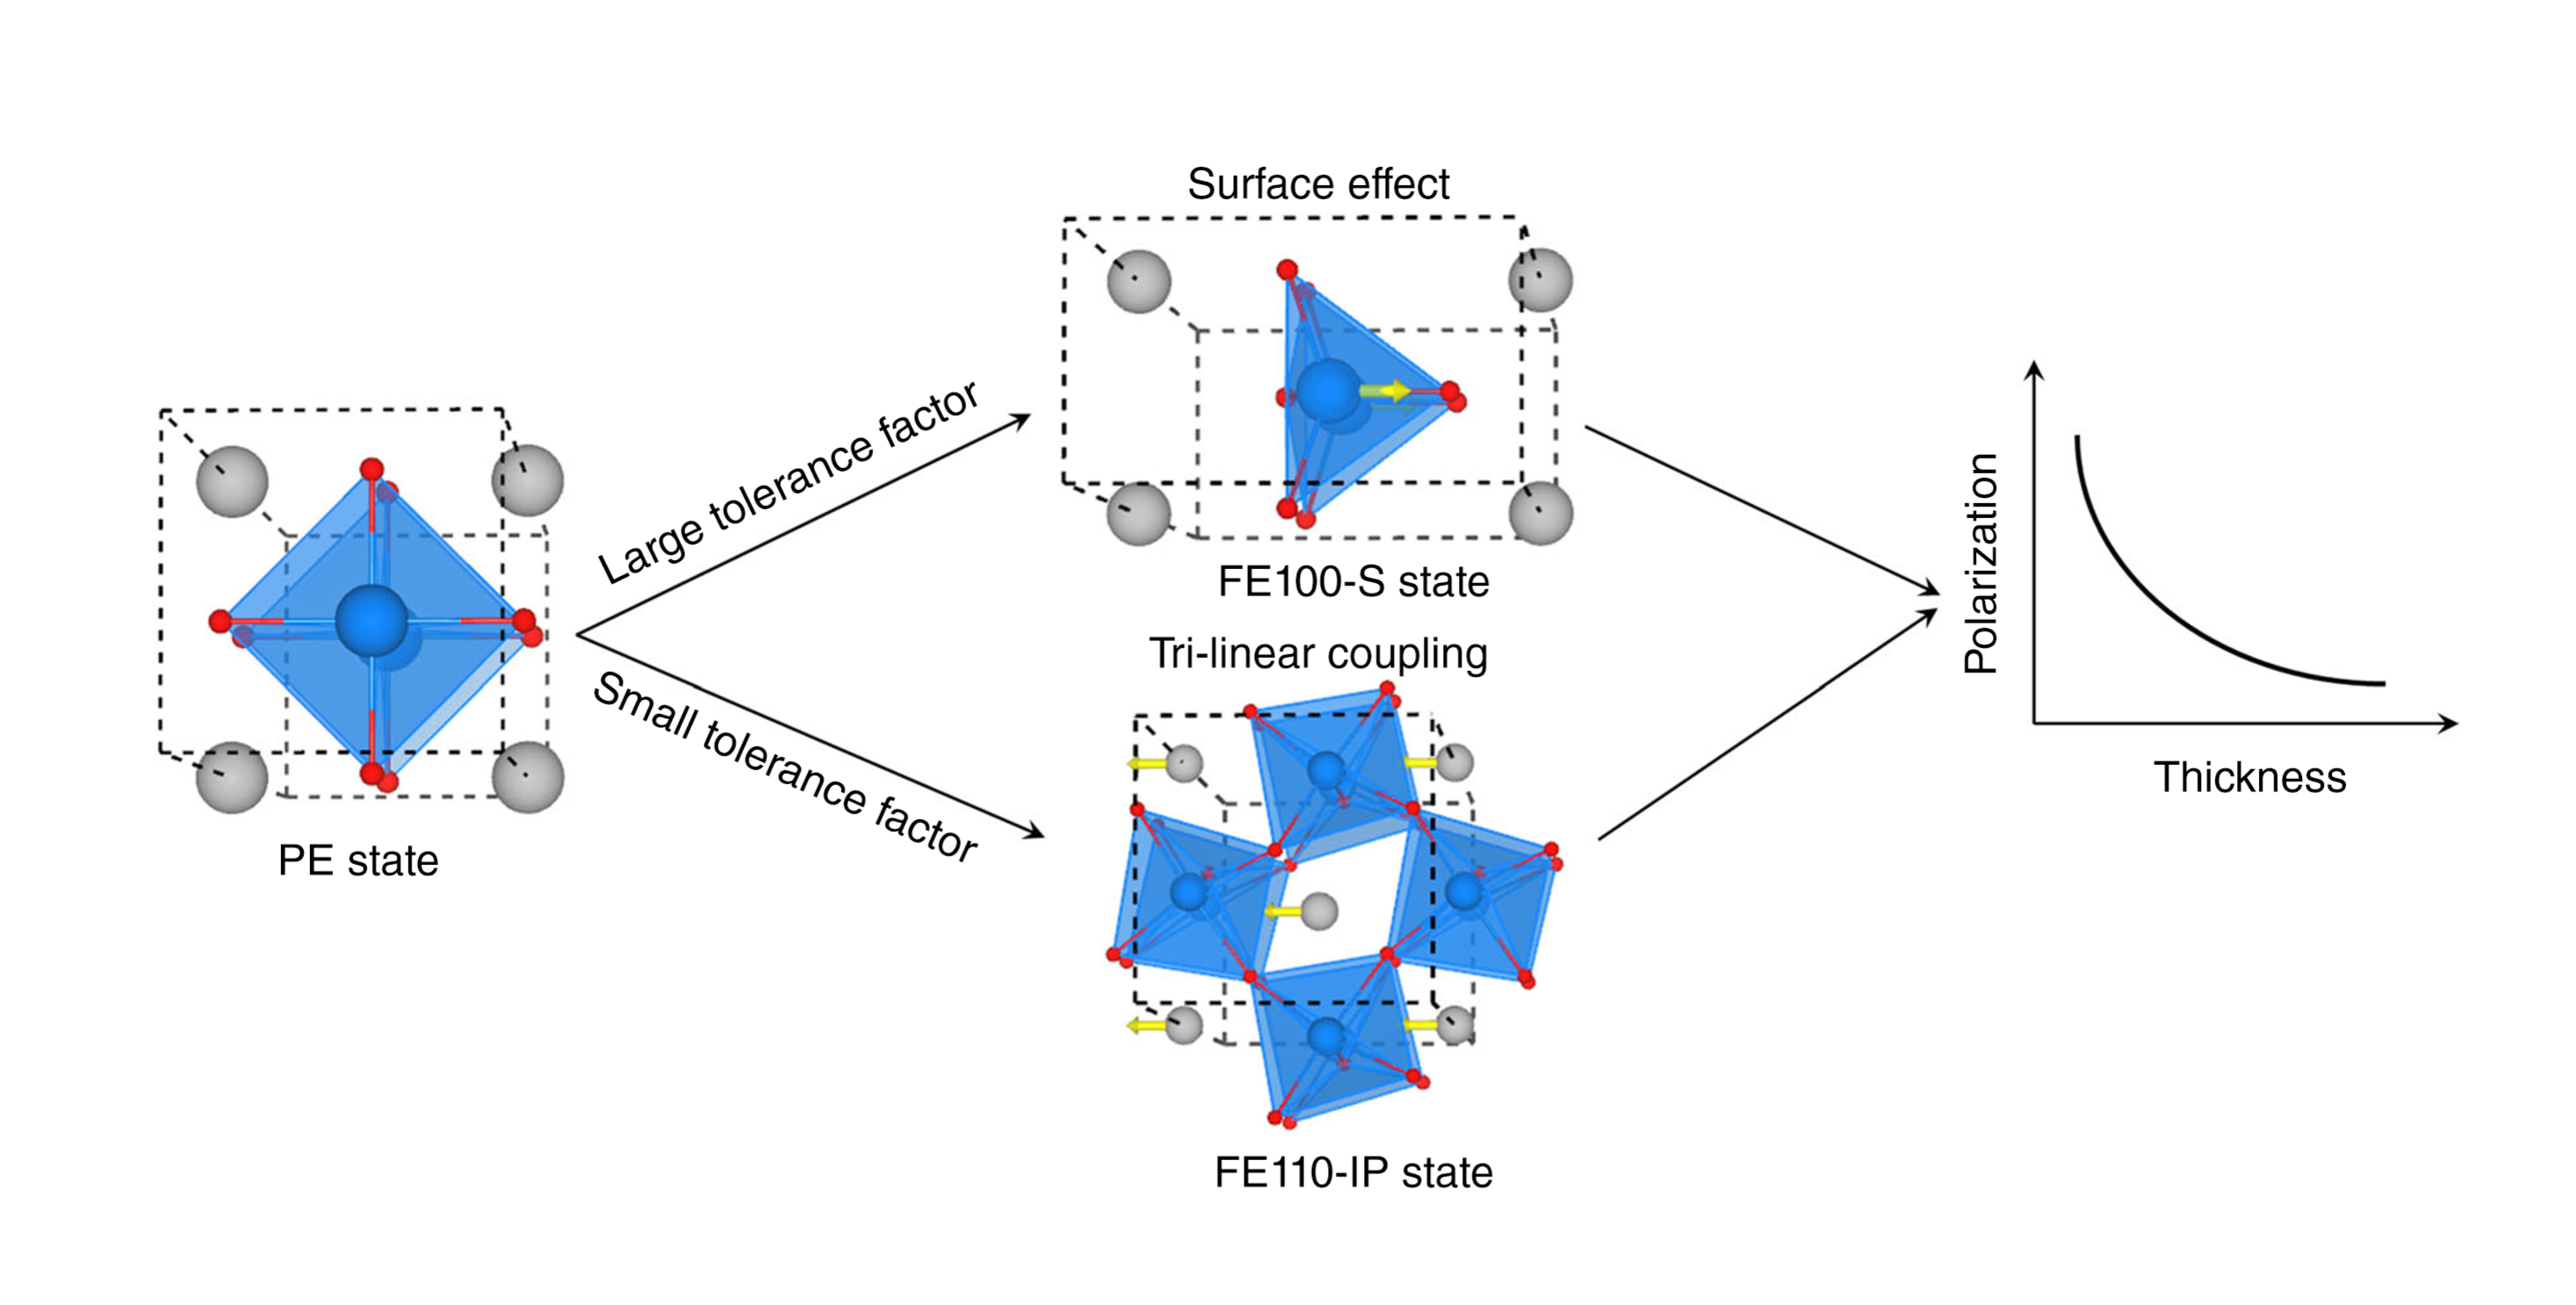
\includegraphics[width=0.8\textwidth]{./pic/014.png}
\caption{二维钙钛矿结构薄膜之中两种不同的氧八面体扭曲结构形成的铁电相,不同的扭曲方式与金属阳离子的半径有关,整个二维体系的铁电性随厚度的减小而增强}

\label{dog014}
\end{figure}

\subsection{基于钙钛矿结构的铁电材料}

在通常的三维材料之中$ABO_{3}$形式的钙钛矿结构通常是铁电压电研究领域的常见材料,在二维条件下,钙钛矿结构的铁电材料有着极大的研究价值。将在三维体系之中表现良好的钙钛矿结构经过降维之后应用在二维材料之中也是一种不错的思路。对于典型的$ABO_{3}$钙钛矿结构,扭曲结构系数$t=(r_{A}+r_{O}/\sqrt{2}(r_{B}+r_{O}))$,是一个衡量钙钛矿结构扭曲形变的一个重要参数,其中r是钙钛矿中各个粒子的经典半径。如果t比一小,氧八面体会发生明显的倾斜以适应扭曲的晶格结构和失调的原子半径比例所造成的键错配。高对称性晶格结构发生扭曲导致对称性降低是产生铁电性的关键。

\begin{figure}[h]
    \centering
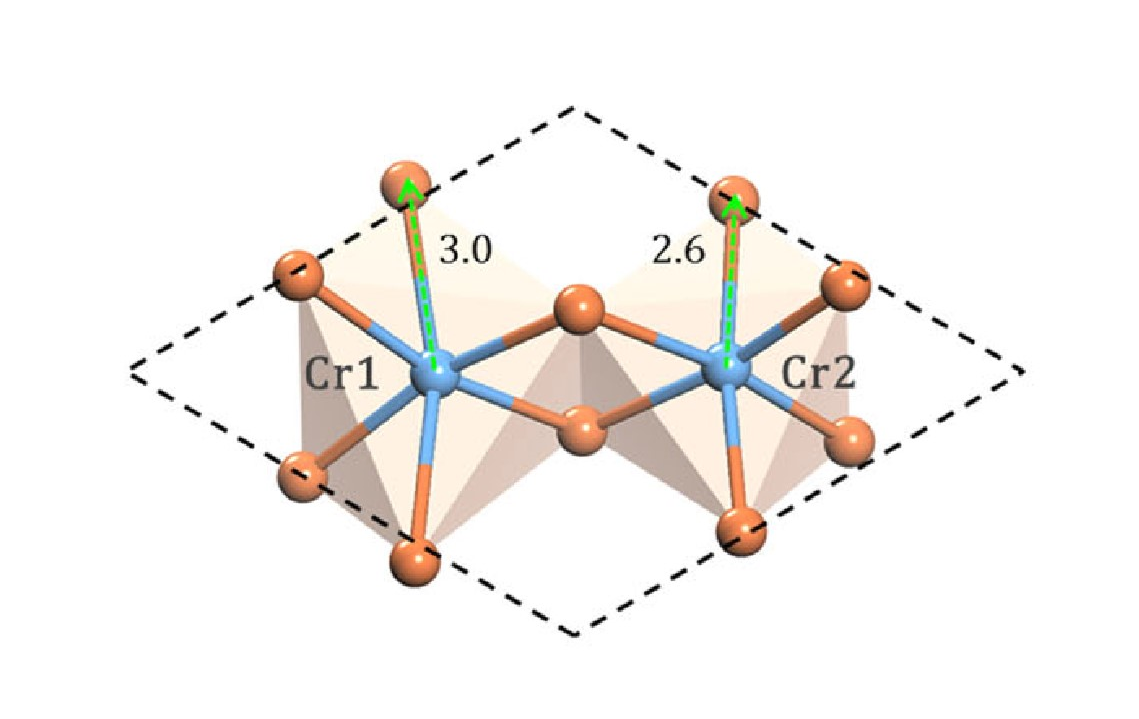
\includegraphics[width=0.8\textwidth]{./pic/010-3.png}
\caption{掺杂电子后的$CrBr_{3}^{0.5-}$结构,电子掺杂使两个$Cr^{3+}$出现差异,地位不在平等,与周围溴离子的键参数发生变化}

\label{dog010-3}
\end{figure}

\section{二维多铁材料的研究背景}

与三维多铁材料一样,二维多铁材料也可以分为两种类型。第一类多铁体的铁磁铁电性质来源不同,第二类二维多铁材料的铁磁铁电性质有着相同的来源。\cite{wang2009multiferroicity:,dong2015multiferroic} 一般来说,第一种的电磁耦合比较弱。而第二类多铁体通常是由于磁有序导致空间的中心对称性破缺,从而出现电极化,这类电磁同源二维多铁材料电磁耦合强,但是电极化很小且温度很低。由于铁电与铁磁效应的内在排斥,很难发现二维多铁材料。

对于已经存在铁电性的二维材料,将其改造为多铁材料最方便有效常用的方法是掺杂磁性元素或过渡金属。对于石墨烯或者其他的一些类似的二维材料,掺杂一些非磁性的元素周期表靠前的元素(H、F),导致费米面附近电子浓度增加,同样也可以产生铁磁性。

目前已将预测或发现了多种的单独存在铁电性与铁磁性的的二维材料。其中二维铁电材料主要有$MoS_{2}$ \cite{yuan2019room-temperature} 、石墨烯 \cite{kan2013high-temperature} 、$SnSe$ \cite{fei2016ferroelectricity} 等二维材料。在二维过渡金属卤化物中也观测到了铁磁性。\cite{huang2017layer-dependent} 通常大部分过渡金属卤化物是磁性半导体或者绝缘体,这给在过渡金属卤化物之中寻找同时存在的铁电性与铁磁性提供了可能。

通过第一性原理计算,卤素修饰磷烯双层可能是带有垂直平面的电极化与可移动磁矩的多铁材料。卤素原子在两层见形成的共价键破坏了两层的对称性,卤素原子在上下两层的结合的改变导致了电极化方向的翻转。磁矩直接来源于卤素原子,每个卤素原子可以提供1$\mu_{B}$的磁矩
,磁矩的方向可以被外加电场的方向改变,这一性质使得这种材料有希望被应用在磁读电写存储器上。

带有乙醚基官能团的锗烯也是一种同时具有铁磁性与铁电性的二维材料。其铁电性来源于极化配体乙醚基在面内的旋转,平面上没有被官能团化的锗原子$p_{z}$轨道上的一个未配对电子提供了1$\mu_{B}$的磁矩。

从另一方面看,对二维铁磁材料进行适当的调整或设计也可以产生多铁性。对于很多过渡金属组成的低维结构,加入一些可以导致对称性破缺的官能团有可能会出现电极化。从实现电极化的翻转难易程度上考虑,通常会添加一些自身带有极化或者强电负性官能团,例如$-F,-Cl,-CN,-NO_{2},=O,-OH \text{或}-COOH $。这类情况通常出现在有机二维网状结构之中,二维$C_{6}N_{8}H$网状结构,质子的输运会导致电极化在两种不同的方向间切换,质子打破了碳氮化物的对称性,使其自旋密度分布各向异性,铁电性与铁磁性之间也发生了耦合。

一般认为铁电性不会出现在具有强铁磁性的金属中,即使金属中存在有微观的电极化,金属中的自由电子会屏蔽掉外电场对自发极化电矩的作用,从而在宏观层面无法表现出铁电性,但在二维材料之中,垂直平面的电极化却很难被面内运动的自由电子屏蔽从而受到垂直平面电场的影响。第一性原理计算表明,具有二维铁磁性的CrN存在垂直平面的电极化,自旋声子耦合使得其内部的铁磁性与铁电性耦合起来。$CrB_{2}$是一种可以用电场调控铁磁性的二维材料,在垂直平面方向施加一个大电场可以使其从反铁磁状态转化为铁磁铁电状态,而一个相对较小的状态可以将其转化回到原来的反铁磁状态。

现在发现的二维多铁材料大多都是第一类多铁材料,第一类多铁材料的电磁耦合强度比较小,为了获取较强的的电磁耦合,需要设计制作第二类多铁材料,即铁电铁磁同源的二维材料。受限于客观条件,这类多铁材料一般很难发现。双过渡金属碳化物$Hf_{2}VC_{2}F_{2}$,是一种第二类二维多铁材料,其120°Y型自旋序打破了空间对称性并产生了一个垂直自旋平面的电极化,但是这个电极化强度过小,只有$ 2.9 × 10^{−7}μC/m$,远小于其他的多铁二维材料。

\begin{table}[!htbp]
    \caption{常见的二维多铁材料}
    \label{tab:dog}
    \resizebox{\textwidth}{!}{
    \begin{tabular}{llllllc}
        \toprule
        
        材料 & 极化强度(pC/m) & 电极化方向 & 磁矩($\mu_{B}$)& FE switch barrier(meV/f.u.) & 转变温度(K) &参考资料 \\
        \midrule
        Phosphorene-halogen&~11&Out-of-plane&1.0&74–590&~572&\cite{yang2017chemically}\\
        Ge-CH2OCH3&~80&In-plane&1.0&~100&—&\cite{kou2018multiferroic}\\
        C6N8H3&6.3–45&In-plane&1.0&70–480&250–700&\cite{tu2017two}\\
        Bilayer Cr2NO2,VS2, MoN2&—&Out-of-plane&0.008–0.09&—&—&\cite{li2017binary}\\
        CrN&6.2&Out-of-plane&3&12&—&\cite{luo2017two}\\
        % CrB&20.9&Out-of-plane&1.5&363&&\\
        CuMP2X6(M = Cr, V; X = S, Se)&0.65–0.79&Out-of-plane&2.0-3.0&27–100&—&\cite{qi2018two}\\
        (CrBr3)2Li&92&In-plane&3.0, 4.0&15&—&\cite{huang2018prediction}\\
        SrMnO3&55μC/cm2&In-plane&—&—&Above 420&\cite{guo2018strain}\\
        Hf2VC2F2&2.9× 10−7&Out-of-plane&2.04&—&313&\cite{zhang2018type}\\


        \bottomrule
    \end{tabular}}
\end{table}

\section{典型的多铁二维材料}

\subsection{溴化铬多铁性产生原理}

二维溴化铬系统中的铁电性可以由电荷排序与轨道排序引发。通过计算表明,在溴化铬二维结构之中掺杂一个电子,通过晶体场理论中的杨-泰勒效应使对称性破缺,两个相邻的$Cr-Br_{6}$单元会产生电荷排序与轨道排序。从而导致二维溴化铬产生多铁性。



三维系统中的电荷排序或者轨道排序都可以独立的产生铁电性,但在二维系统之中,单独的电荷排序并不一定引起对称性的破缺,从而产生电极化。\cite{zhou2014carrier}没有掺杂的二维溴化铬是没有极化现象的铁磁体,当掺杂空穴时对称性没有被破坏,不会产生极化现象。但掺杂电子时,JT效应会使相邻的Cr原子产生不同的能级分裂,导致电子的分布不同,从而产生铁电性。从能带论上面来看,掺杂电子会使费密能级提高,从而使Cr-e态被部分占据,进而使JT扭曲效应出现,破坏对称性。\cite{BENGEL199595} 

\begin{figure}[h]
    \centering
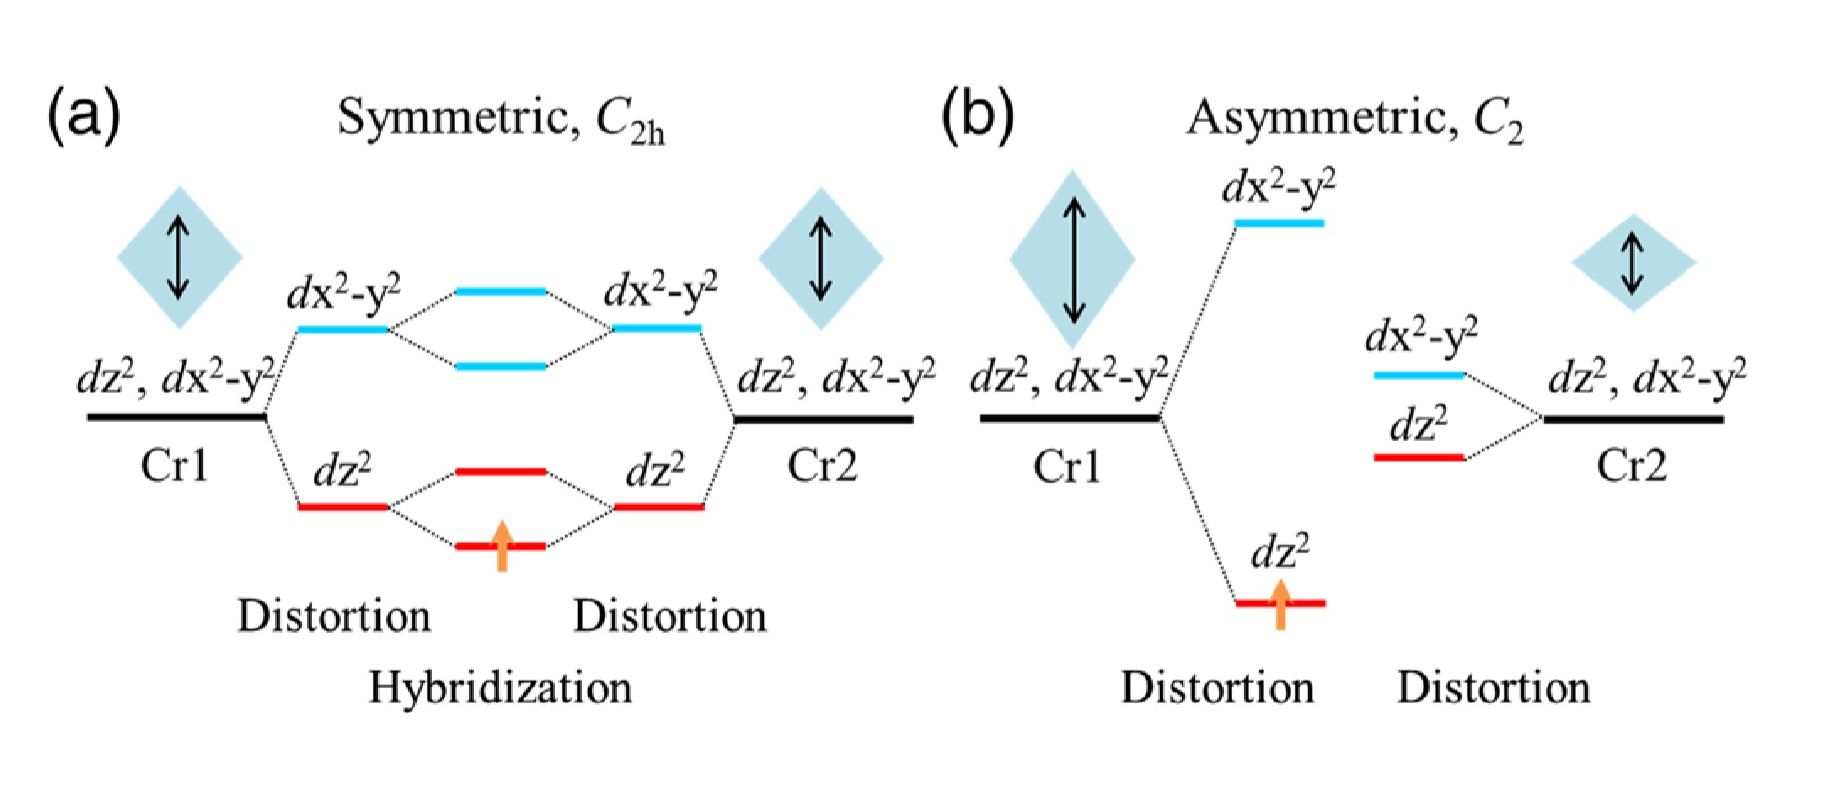
\includegraphics[width=0.8\textwidth]{./pic/011-2.png}
\caption{在不同对称性破缺下,JT效应产生的简并分裂情况不同}

\label{dog011-2}
\end{figure}

在二维溴化铬之中,一个平行四边形基元内部有两个铬离子。在未经掺杂的溴化铬二维层状结构中,只存在铁磁性,没有极化现象。在掺杂空穴的$CrBr_{3}^{x+}$之中,垂直二维平面的对称性没有被破坏。而在电子掺杂的$CrBr_{3}^{x-}$之中,JT效应会使晶格空间结构发生畸变,然后在$C_{2}$对称轴(面内对称轴,详见图)方向,出现电极化。从能带论上面看来,空穴掺杂会使系统的费米面降低,到达Br-p轨道附近,这样就不能引发JT效应使对称性破缺。掺杂电子时,费米面会升高,到达Cr-e轨道附近,所引起的JT扭曲效应会使对称性破缺,从而产生出一个允许电极化存在的特殊方向。对于$CrBr_{3}^{0.5-}$,在平行四边形基元内部,两个Cr并不是完全等价的,Br-Cr键长在垂直于平面的方向有着大约0.4A的差距,这在普通的过度金属卤化物是十分异常的。通过计算表明,$CrBr_{3}^{0.5-}$这种反对称的畸变比对称性的畸变和没有产生畸变情况下能量都要低。

$CrBr_{3}^{0.5-}$的电极化来源于JT效应导致的对称性破缺,其铁磁性则来源于作为过渡金属元素的铬离子,铁电性与铁磁性的耦合最终还是要依靠自旋轨道耦合来解释。铁电性的来源是JT效应,归根结底还是原子轨道叠加杂化组合引起的电子密度分布的变化,铁磁性的来源与其他过渡金属元素组成的物质类似,归根结底是电子自旋,这样看来自旋轨道耦合是连接铁磁性与铁电性的关键。

对于$CrBr_{3}^{0.5-}$,JT效应造成能级分裂有两种,一种是对称的,另一种是反对称的,在对称的$C_{2h}-CrBr_{3}^{0.5-}$之中,两个$Cr-Br_{6}$单元发生同样的分裂:一个更高能量的$dx^{2}-y^{2}$轨道和一个更低能量的$dz^{2}$状态。掺杂进来的多的那个电子占据在两个$Cr-dz^{2}$轨道的超杂化态。两个Cr原子完全等价。在反对称的$C_{2}-CrBr_{3}^{0.5-}$,两个$Cr-Br_{6}$扭曲的程度不同,所造成的能级分裂也不同,这就导致了两个Cr的低能级轨道很难进行超杂化,只能占据Cr1的低能量$dz^{2}$。再加上3d轨道的定域性比较强,电子近似可以看作只停留在一个Cr附近。通过对这两种掺杂电子的分裂方式进行计算,反对称方式能量低大约0.8电子伏,这就导致在$CrBr_{3}^{0.5-}$系统中更偏向出现反对称JT效应。

在真实的二维材料之中掺杂电子有很多方法,可以采用合适的基底、掺杂金属或离子。目前已经可以在FeSe薄片中掺杂高比例锂离子进行电子掺杂。\cite{lei2017tuning} 选择$(CrBr_{3})_{2}Li$或许是可行的。 同样对于其他的卤族元素,如氯、碘等元素,与$CrBr_{3}$有着相似的原子电子结构,也具有多铁性。这样的理论在其他的过渡金属卤化物上也适用。

\section{基于四族元素的一硫族化合物的多铁二维材料}

第四主族的一些元素的与S、Se等形成的二维层状化合物具有面内的在室温下可以稳定存在的多铁性,与其他多铁材料不同的是,这类材料的铁性质不是常见的铁磁性与铁电性性,而是铁电性与铁弹性。\cite{wang2017two}\cite{ISI:000088490500004}这类材料不仅有多铁性,而且对可见光谱有着各向异性的强吸收,这意味着有可能透过光场对材料的多铁性质进行调控。这种铁电性、铁弹性与光学性质耦合的多铁二维材料在制备二维可调控多铁器件与铁电存储器方面有着巨大的潜力。
\begin{figure}[h]
    \centering
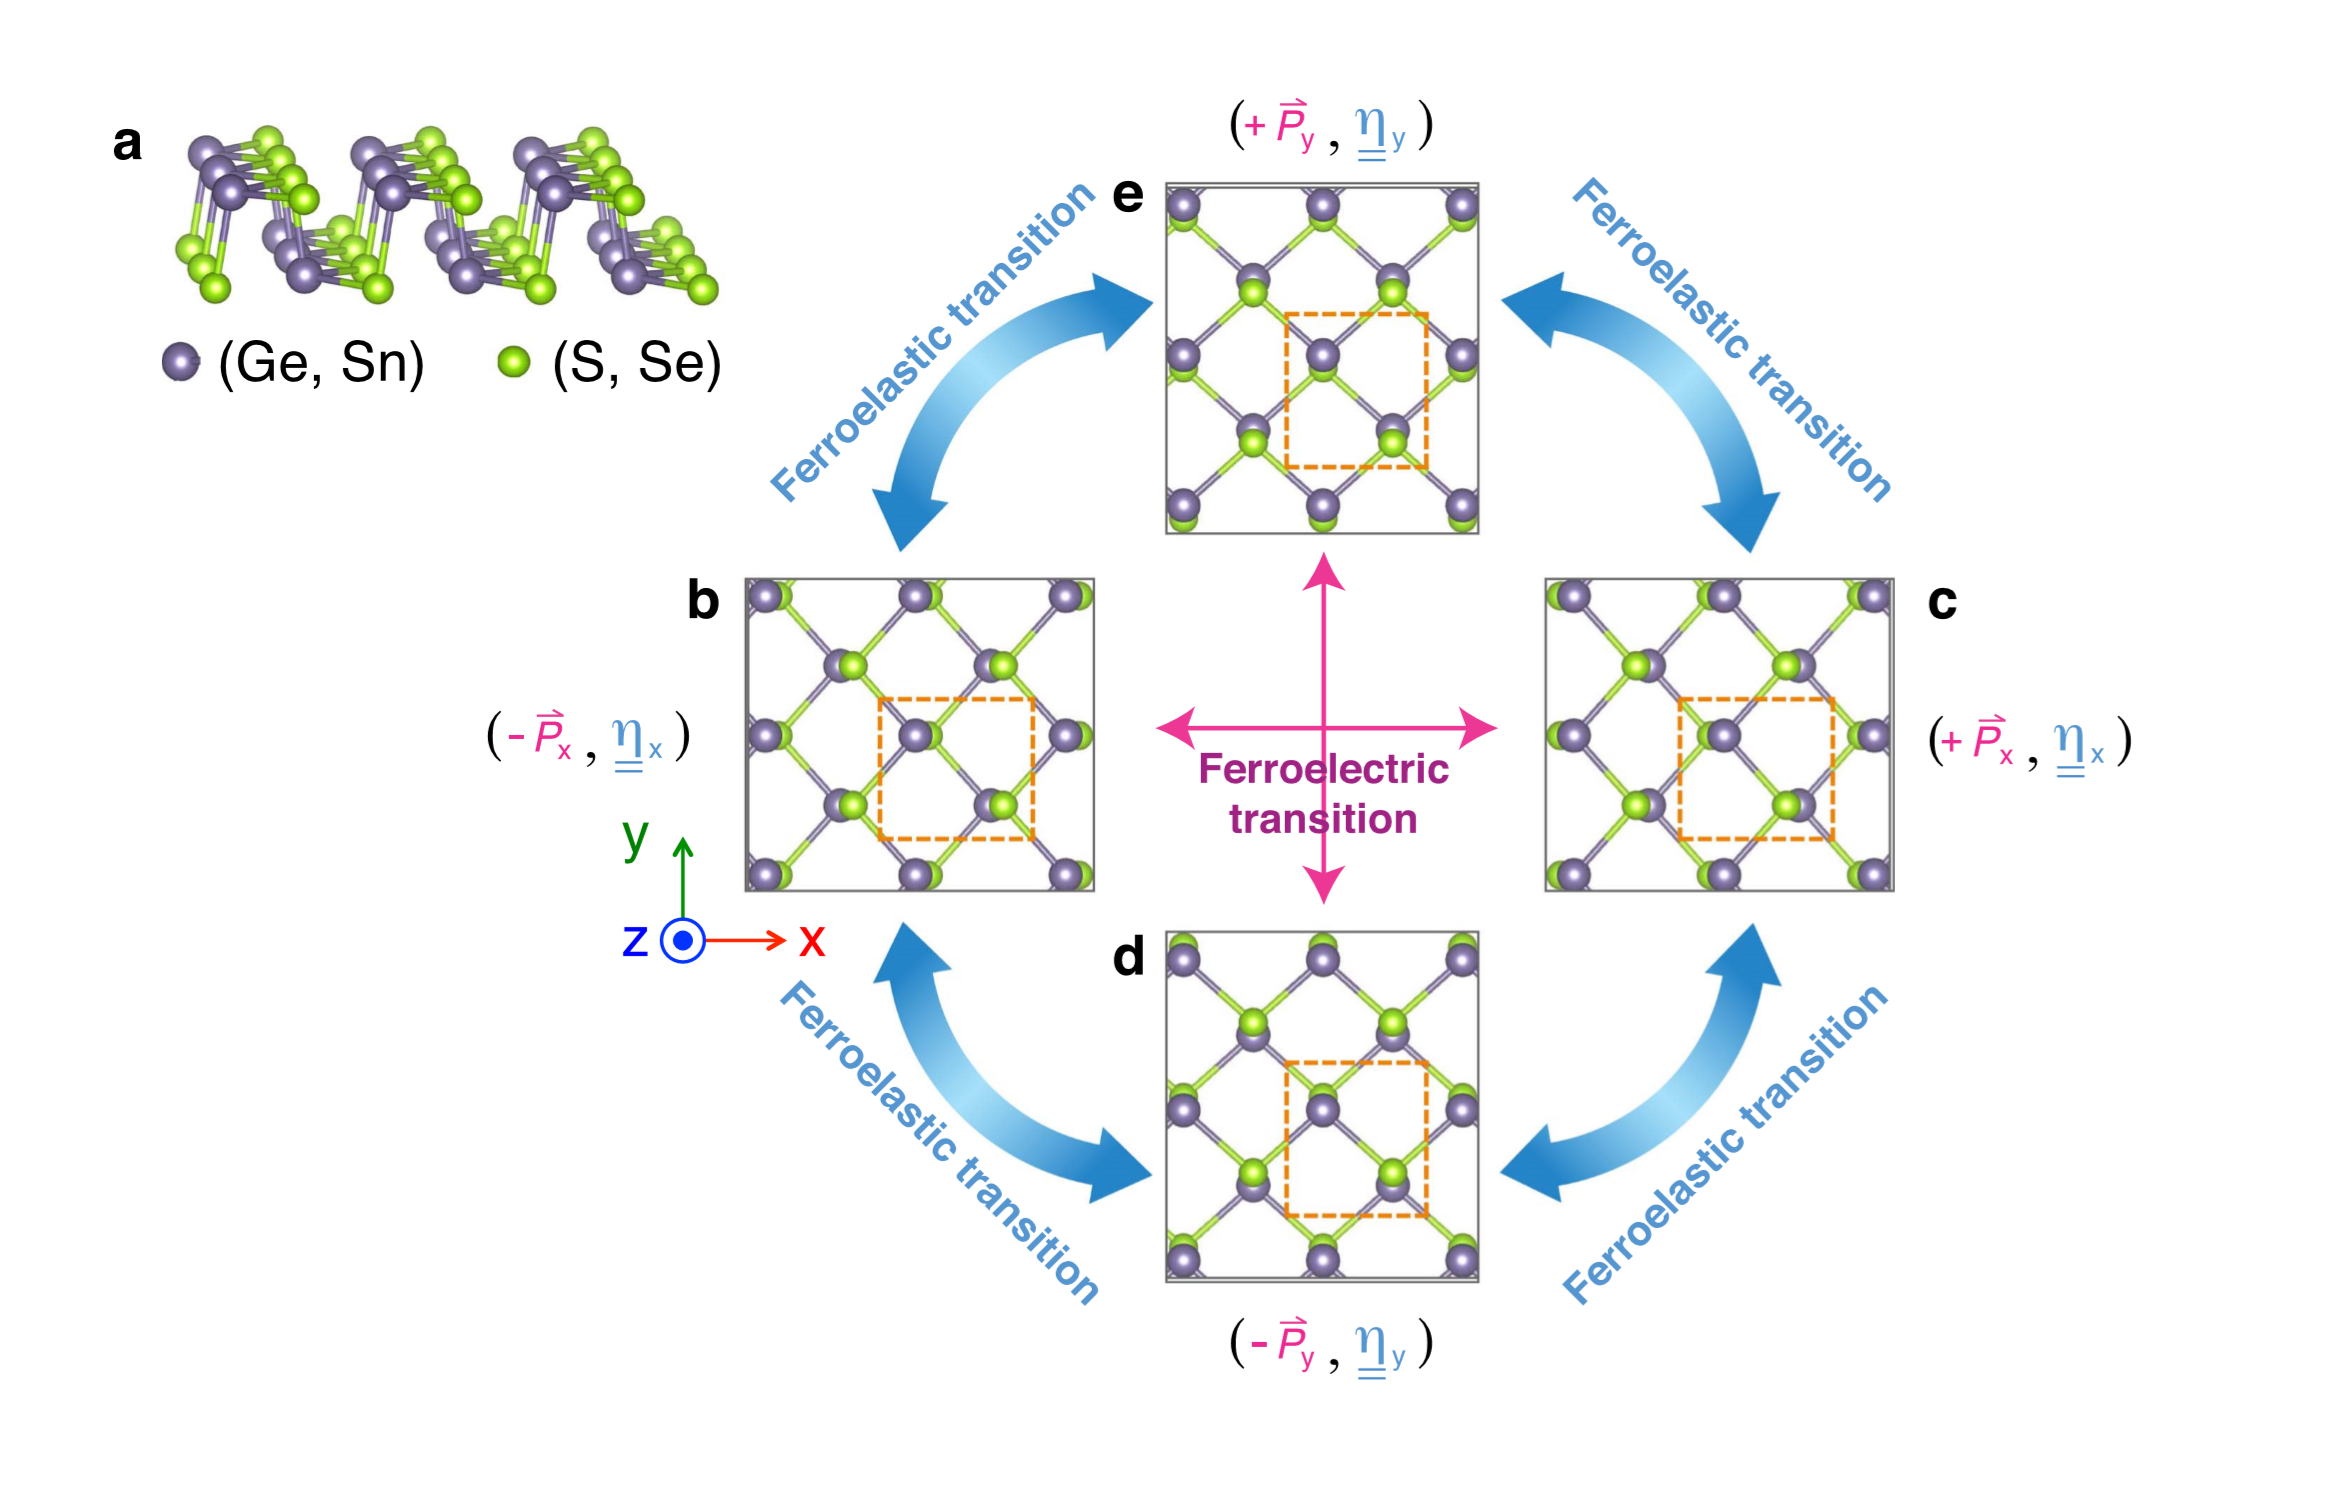
\includegraphics[width=0.8\textwidth]{./pic/018.png}
\caption{MX二维分子层状结构与面内的铁电性与铁弹性\ 分子层内部有四种电极化方向,沿着X轴有两种电极化状态$P_{x}\text{和}-P_{x}$,沿着Y轴也有两个电极化状态$P_{y}\text{和}-P_{y}$ \ 有两种铁弹性状态$\eta_{x}\text{和}\eta_{y}$这四种状态可以通过铁电性与铁弹性进行相互转化}

\label{dog018}
\end{figure}

作为一大类二维多铁材料\cite{ISI:000230853300010},四族元素的一硫族化合物(主要包括GeS, GeSe, SnS ,SnSe等)有着相似的结构,同样拥有强耦合的多铁性。\cite{ISI:000318143300005}\cite{ISI:000309505400023}可以认为。多铁性在这些材料中是普遍存在的。这类二维材料的铁弹性与二维晶格两个垂直方向的形变有关,晶格扭曲导致内部正负电荷中心发生位移,进而导致材料内部电极化发生变化,铁弹性是与铁电性直接耦合的,这支持了采取外场对另一种铁性质进行调控的可能。

\subsection{铁弹性与自发应变}

四族元素的一硫族化合物通常可以表示为MX,其中M可以是Ge、Sn,X是S 、Se。以GeSe为例,GeSe的单层结构如图所示,其铁弹性起源于其晶格结构沿x和y方向发生自发弛豫,晶格移动形变的方向不同。\cite{ISI:000363915300044}通过计算表明,稳定的层状机构并不是在XY方向对称的,在一个方向压缩与另一个方向拉伸。压缩与拉伸的方向不同可以分成两个相,二既不拉伸又不压缩的中间状态能量比较高,这就形成了一个势垒。如果有外加影响如外场或者外加应力,会是一个相越过中间的势垒转化到另一个相。微观机构的晶格参数的改变在宏观层面表现出来就是几何外形与尺寸的改变。从对称性来看。在平面内部XY方向的对称性被破坏,其中一个方向变得特殊起来,各种铁性质的出现与对称性的破缺有着密切的关系。

\begin{figure}[h]
    \centering
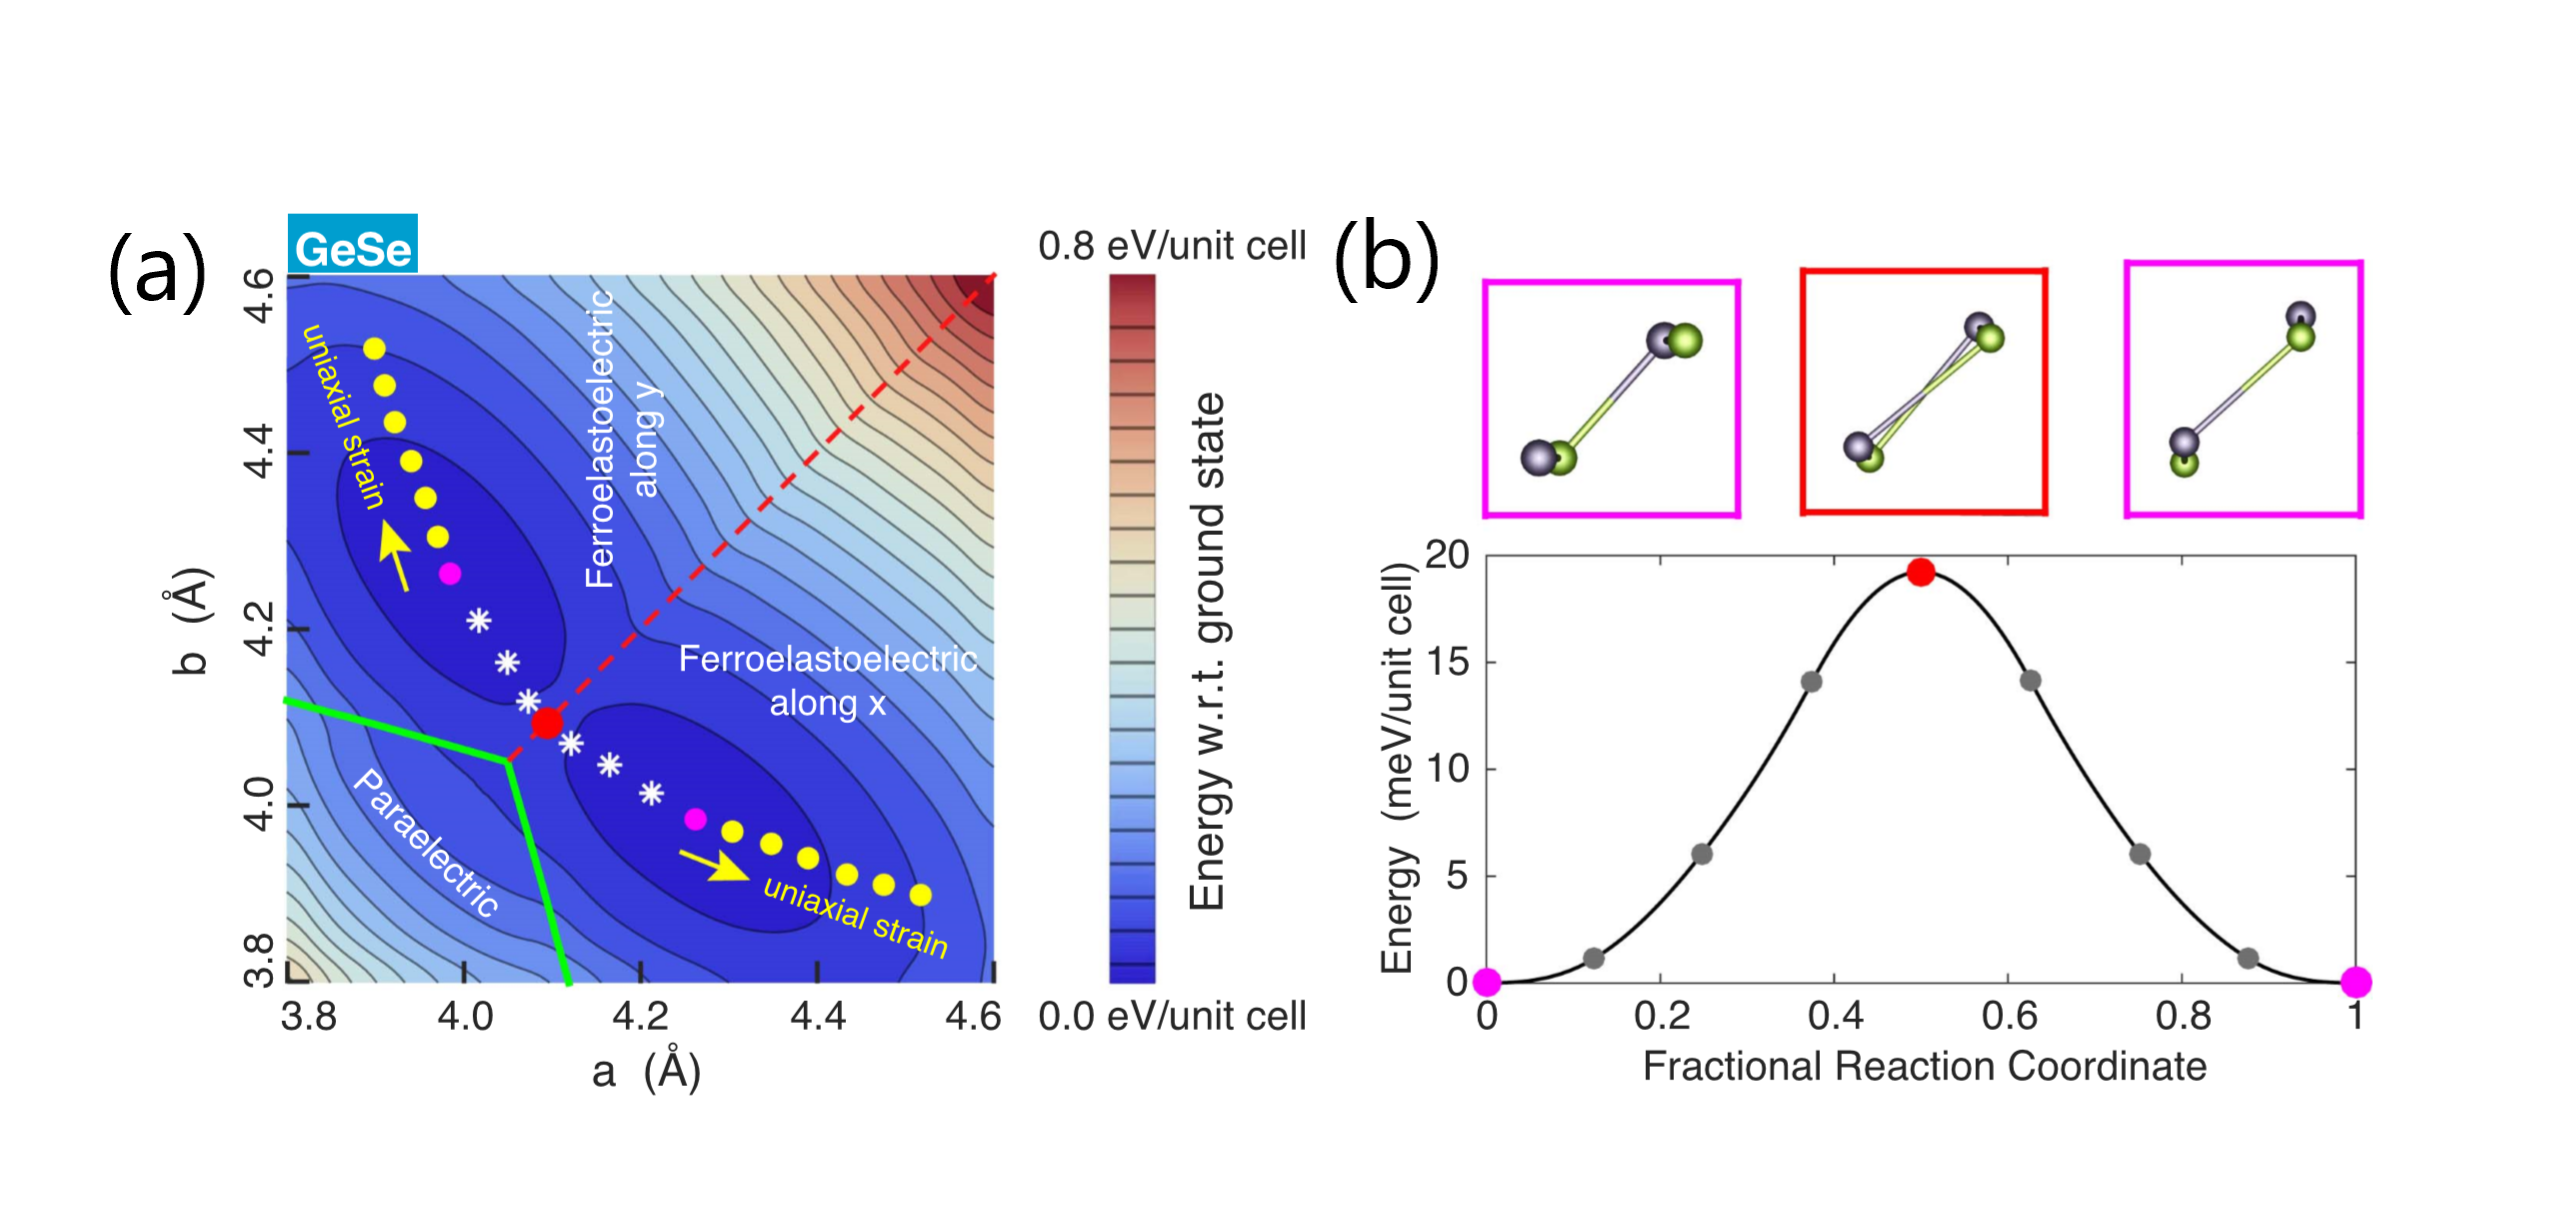
\includegraphics[width=0.8\textwidth]{./pic/017.png}
\caption{(a)不同晶格常数下GeSn的总能量\ 可以从图上看到,有着一个高对称性顺弹性相,位于势能的曲面的鞍点,并不是一个能量最低的稳定态,两个稳定态是两个不同的铁弹性太,具有自发的应变。(b)两个铁弹性态之间转换的最低能量路径,从图中可以看出,两种状态之间的转换并没有经过高对称性的顺弹性状态,而是通过层状结构上下原子位置的相对转动从一种状态转化到另一种状态。}

\label{dog017}
\end{figure}

进一步的计算表明,对称性较高的顺弹性的态是亚稳态其晶格常数可以用矩阵$\bm{H}_{ref}=\begin{bmatrix}
    &4.1&0\\
    &0&4.1
\end{bmatrix}$表示。选取高对称顺弹性状态$\bm{H}_{ref}$作为参考,两种低对称性的状态分别为$\bm{H}_{x}=\begin{bmatrix}
    &4.26&0\\
    &0&3.98
\end{bmatrix}$和$\bm{H}_{y}=\begin{bmatrix}
    &3.98&0\\
    &0&4.26
\end{bmatrix}$
相对于基准状态,两种状态的转换应变矩阵:
\begin{equation}
    \begin{split}
        &\eta_{x}=\frac{1}{2}([H_{ref}^{-1}]^{T}H_{x}^{T}H_{x}H_{ref}^{-1}-\bm{I})\\
        &\eta_{y}=\frac{1}{2}([H_{ref}^{-1}]^{T}H_{y}^{T}H_{y}H_{ref}^{-1}-\bm{I})\\
        &\eta_{x}=\begin{bmatrix}
            0.041&0\\
            0&-0.027
        \end{bmatrix}\\
        &\eta_{y}=\begin{bmatrix}
            -0.027&0\\
            0&0.041
        \end{bmatrix}
    \end{split}
    \label{eq:txxb}
\end{equation}
对于$\eta_{x}$,这表示在X方向发生了4.1\%的拉伸,在Y方向发生了2.7\%的压缩。同样地对于$\eta_{y}$,这表示在Y方向发生了4.1\%的拉伸,在X方向发生了2.7\%的压缩。虽然在两种铁弹性相之间有着一个顺弹性势垒,但在这两种铁弹性状态转变时,却不会经历中间的顺弹性状态。而是通过两种原子的相对旋转实现的。

\subsection{铁电性与自发极化}
虽然铁电与铁弹性有着密切的关系,都存在着空间范畴上的对称性破缺,但这两点又有着区别与不同。铁电性是正负电荷中心自发偏离,形成空间中的电偶极子与自发极化。在自发极化方向翻转时不一定会产生宏观层面的晶格形变,反之在晶格结构发生变化时,自发极化、正负电荷中心也不一定随之发生变化。对于像GeSe这样铁弹性与铁电性强耦合的材料,其内部有着及其密切的关系。基于量子绝热定理,可以通过几何相位导出自发极化强度的表达式:
\begin{equation}
    \begin{split}
        \bm{P}_{s}&=\bm{P}^{f}-\bm{P}^{i}\\
        &=\frac{1}{\Omega}\sum_{j}(q^{f}\bm{r}^{f}-q^{i}\bm{r}^{i})-\frac{2ie}{(2\pi)^{3}}\sum_{n}^{occ} [ \int_{BZ}d^{3} \bm{k} e^{-i\bm{k \cdot R}} \\
        & \times \langle u^{f}_{n \bm{k}} | \frac{\partial u_{n \bm{k}}^{f}}{\partial \bm{k}} \rangle - \langle u^{i}_{n \bm{k}} | \frac{\partial u^{i}_{n \bm{k}}}{\partial \bm{k}} \rangle ]
    \end{split}
    \label{eq:}
\end{equation}
其中i,j分别表示在量子绝热理论中的出=初状态与末状态。
通过第一性原理计算,GeSn具有强烈的铁弹性与铁电性的耦合。例如当单轴应变增大6\%时自发极化从357pC/m增加到430pC/m。

\subsection{各向异性的光学性质}

通过应用DFT等手段对GeSn等材料的能带结构的计算,MX单分子膜是具有2.6ev-1.1ev间接带隙的二维半导体材料。二维平面内的电极化会导致在二维分子平面内部不同方向的介电常数不同,会导致对不同偏振方向的光产生不同的响应。利用这一点可以采用可见光照射的方式读取二维材料的铁电、铁弹性状态。
\begin{figure}[h]
    \centering
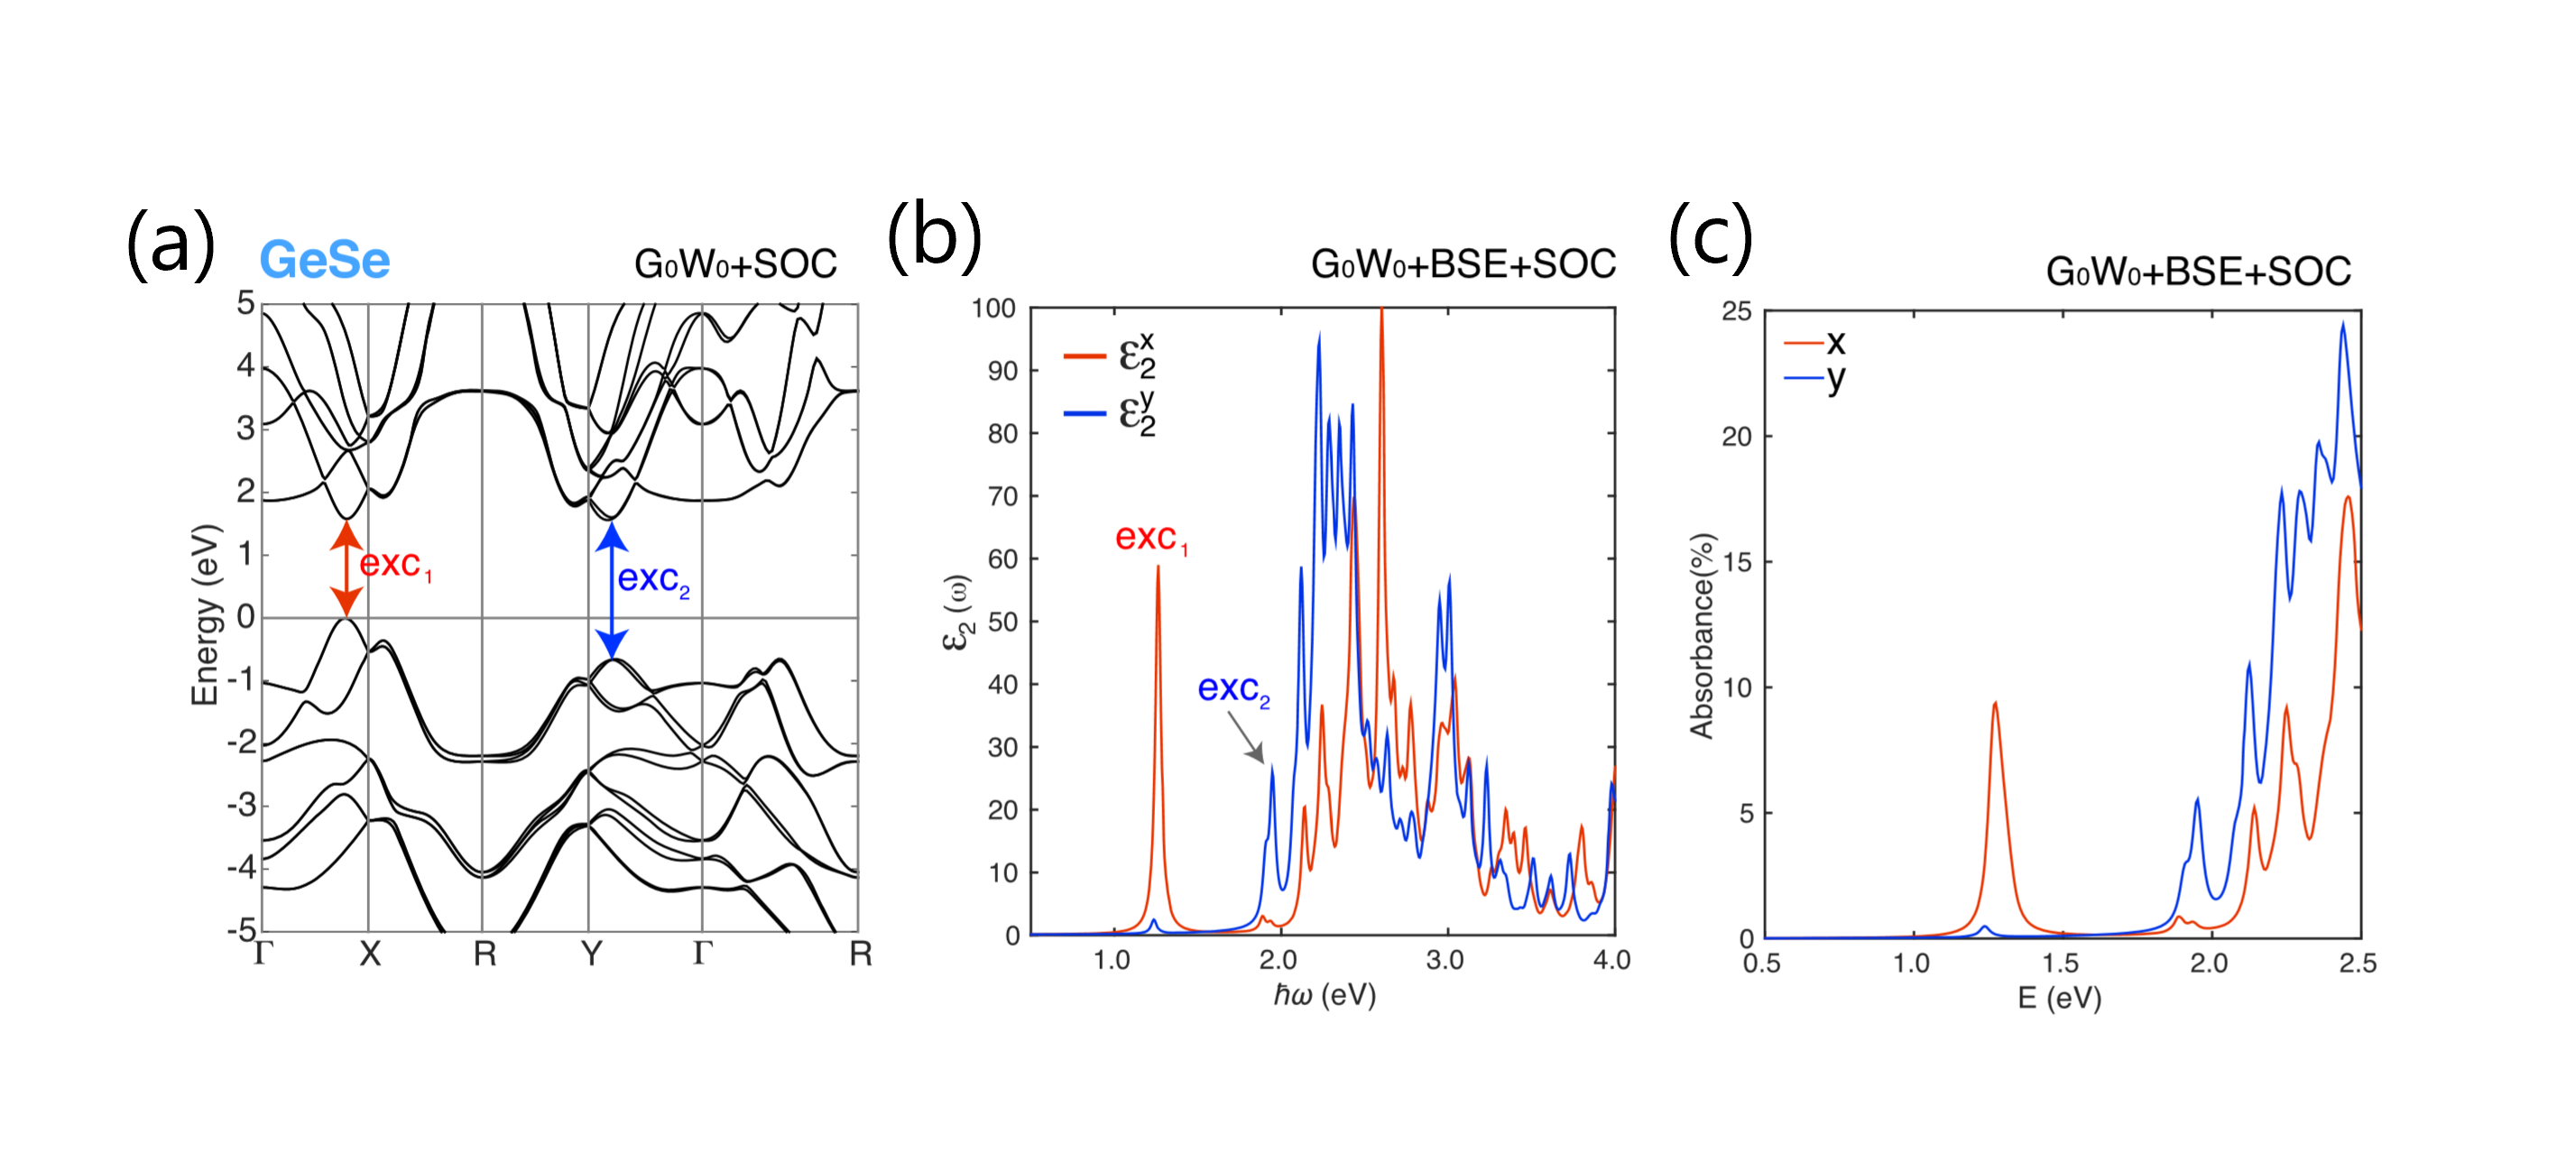
\includegraphics[width=0.8\textwidth]{./pic/019.png}
\caption{(a)在$G_{0}W_{0}$近似下得到的GeSn能带图,从图中可以看到二维层状GeSn是一种半导体,结构上的各向异性导致其对光的相应也具有各向异性(b)通过能带计算出的介电常数,有着明显的各向异性(c)单层GeSn的光吸收度}

\label{dog019}
\end{figure}

\section{双金属三卤化物}
对于铁电性与铁磁性的多铁材料,其多铁性的研究核心是在铁电性与铁磁性的耦合。二维双金属三卤化物是一种新型通过理论计算发现的二维多铁材料。$ReWCl_{6}$是一种单相同时具有铁磁性与铁电性的第一类二维多铁材料。\cite{xu2020electrical}由于铁磁性与铁电性来源不同,第一类多铁材料与第二类相比电磁耦合要弱。这种材料具有面内的电极化与铁磁性和反铁磁性两种磁性状态,而且通过外加电场同时改变电极化方向与两种铁磁相之间的切换。是一种可以通过电场控制磁场的二维多铁材料。

\subsection{结构与铁电性}

\begin{figure}[h]
    \centering
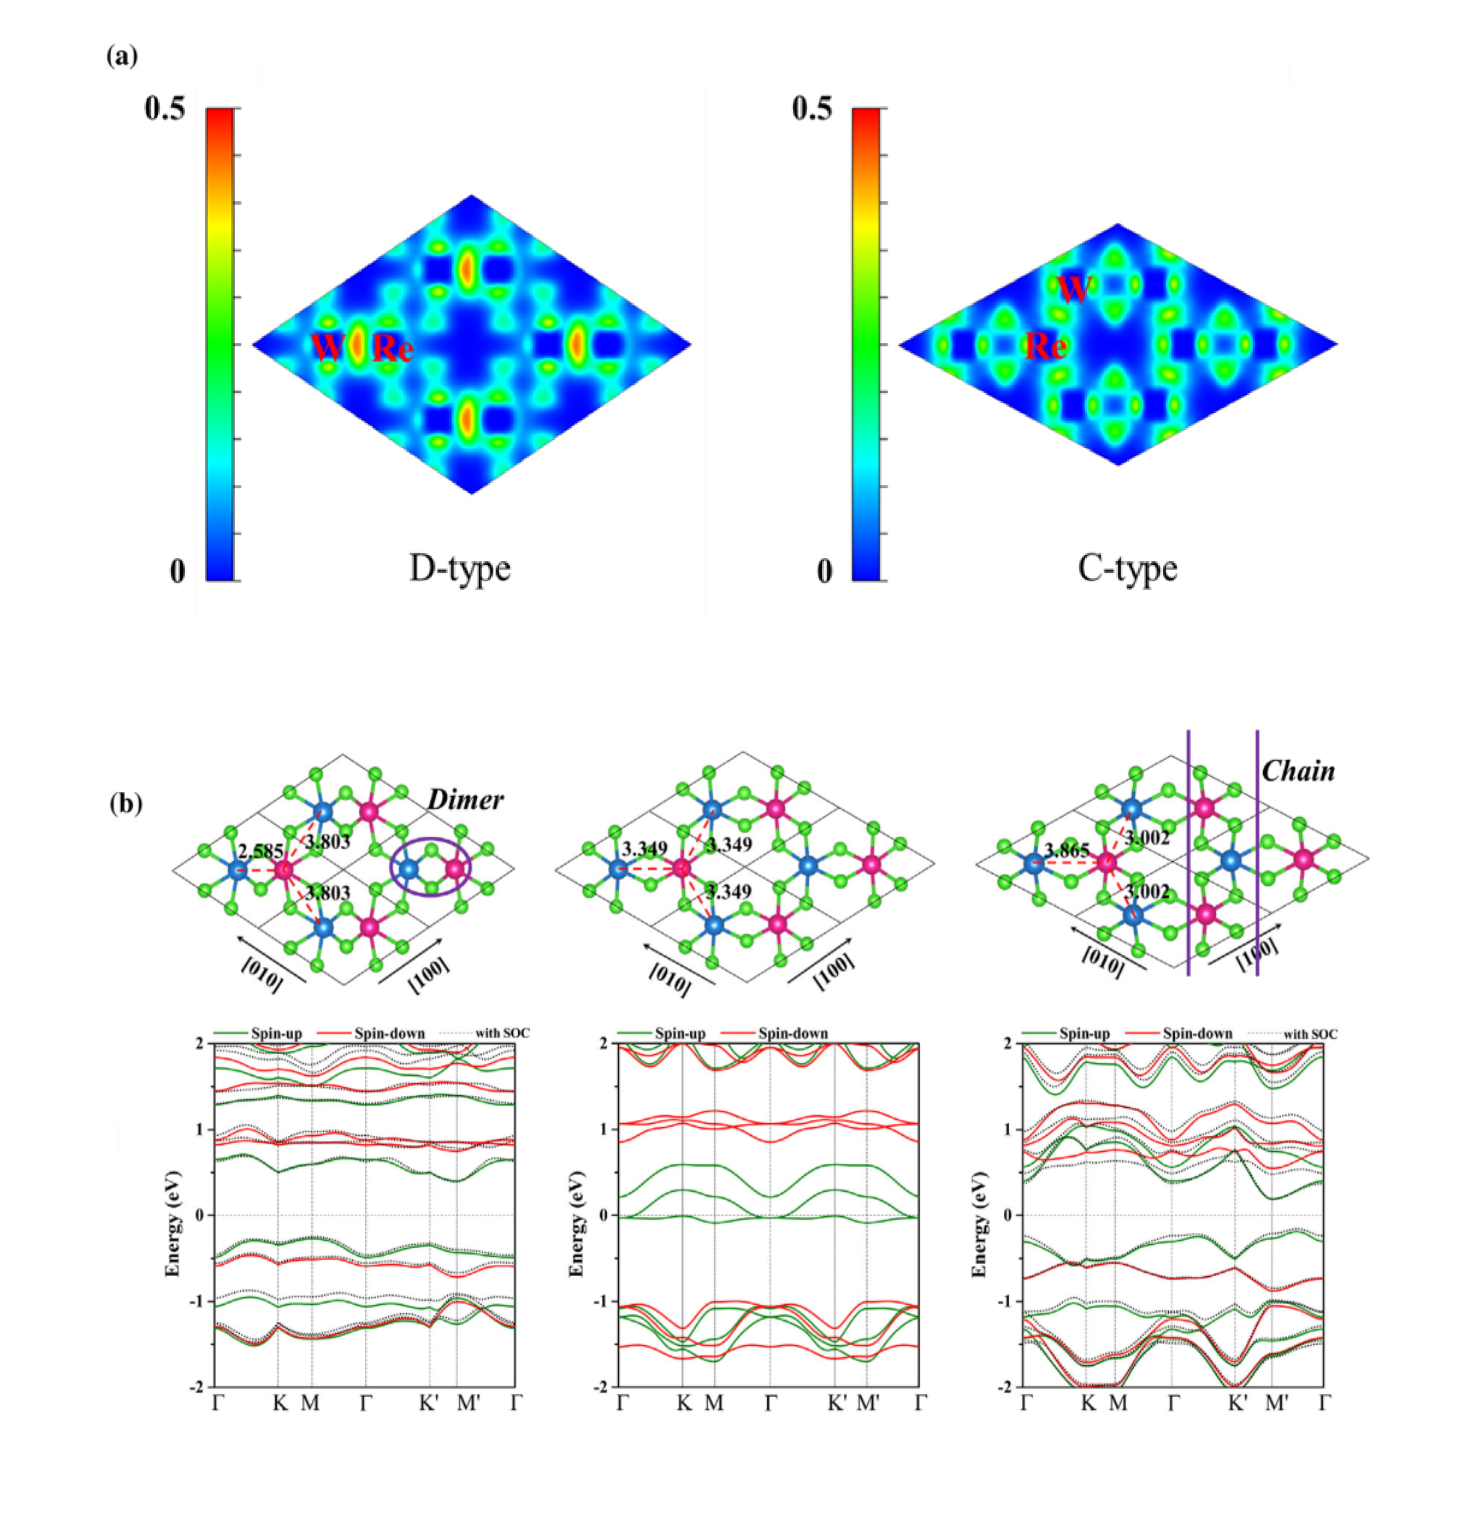
\includegraphics[width=0.8\textwidth]{./pic/021.png}
\caption{(a)D型和C型电子分布图\ 从图中可以明显看出两种结构的电极化方向、强度不同\ (b)$ReWCl_{6}$三种结构(D型、C型与高对称的$C_{3}$型)的俯视图与能带结构 \ 其中蓝色代表W原子、红色代表Re原子、绿色代表氯原子,层状结构之中的W-Re聚合体与W-Re-W-Re链条已被标出。从三种不同结构的能带图上可以看出,D型、C型均是有着不同带隙的半导体,高对称的$C_{3}$型是导体。通过虚线所示的考虑自旋轨道耦合后的两种计算结果后的差别,自旋轨道耦合对体系的影响不大,不是影响$ReWCl_{6}$多铁性性质的决定性因素。}

\label{dog021}
\end{figure}

与之前提到的过渡金属卤化物类似,二维双金属卤化物层状结构也是类似的三角形结构。对于三角形结构,一般有$C_{2}\text{、}C_{3}$两种对称性。铁电性的出现通常意味着空间对称轴的破坏与对称性的降低。对于二维晶体结构,对称性的降低通常是由于某些原因$C_{3}$对称性不复存在,这样在$C_{2}$对称轴这个方向就会成为一个特殊方向,这个特殊的方向往往就是电极化的方向。如图所示,原子位移与结构扭曲导致$ReWCl_{6}$的对称性被破坏,由$C_{3}$高对称状态转化为两种$C_{2}$低对称状态,分别为D型与C型。D型C型两种结构由于原子移位不同,产生两种相反的自发极化方向。这两种类型的微观结构不同,其表现出来电磁性质也不同。因此在通过外加电场对这两种铁电状态进行反转时,其磁性性质也会随之改变,可以通过外加电场的方式改变$ReWCl_{6}$的磁性质。

\begin{figure}[h]
    \centering
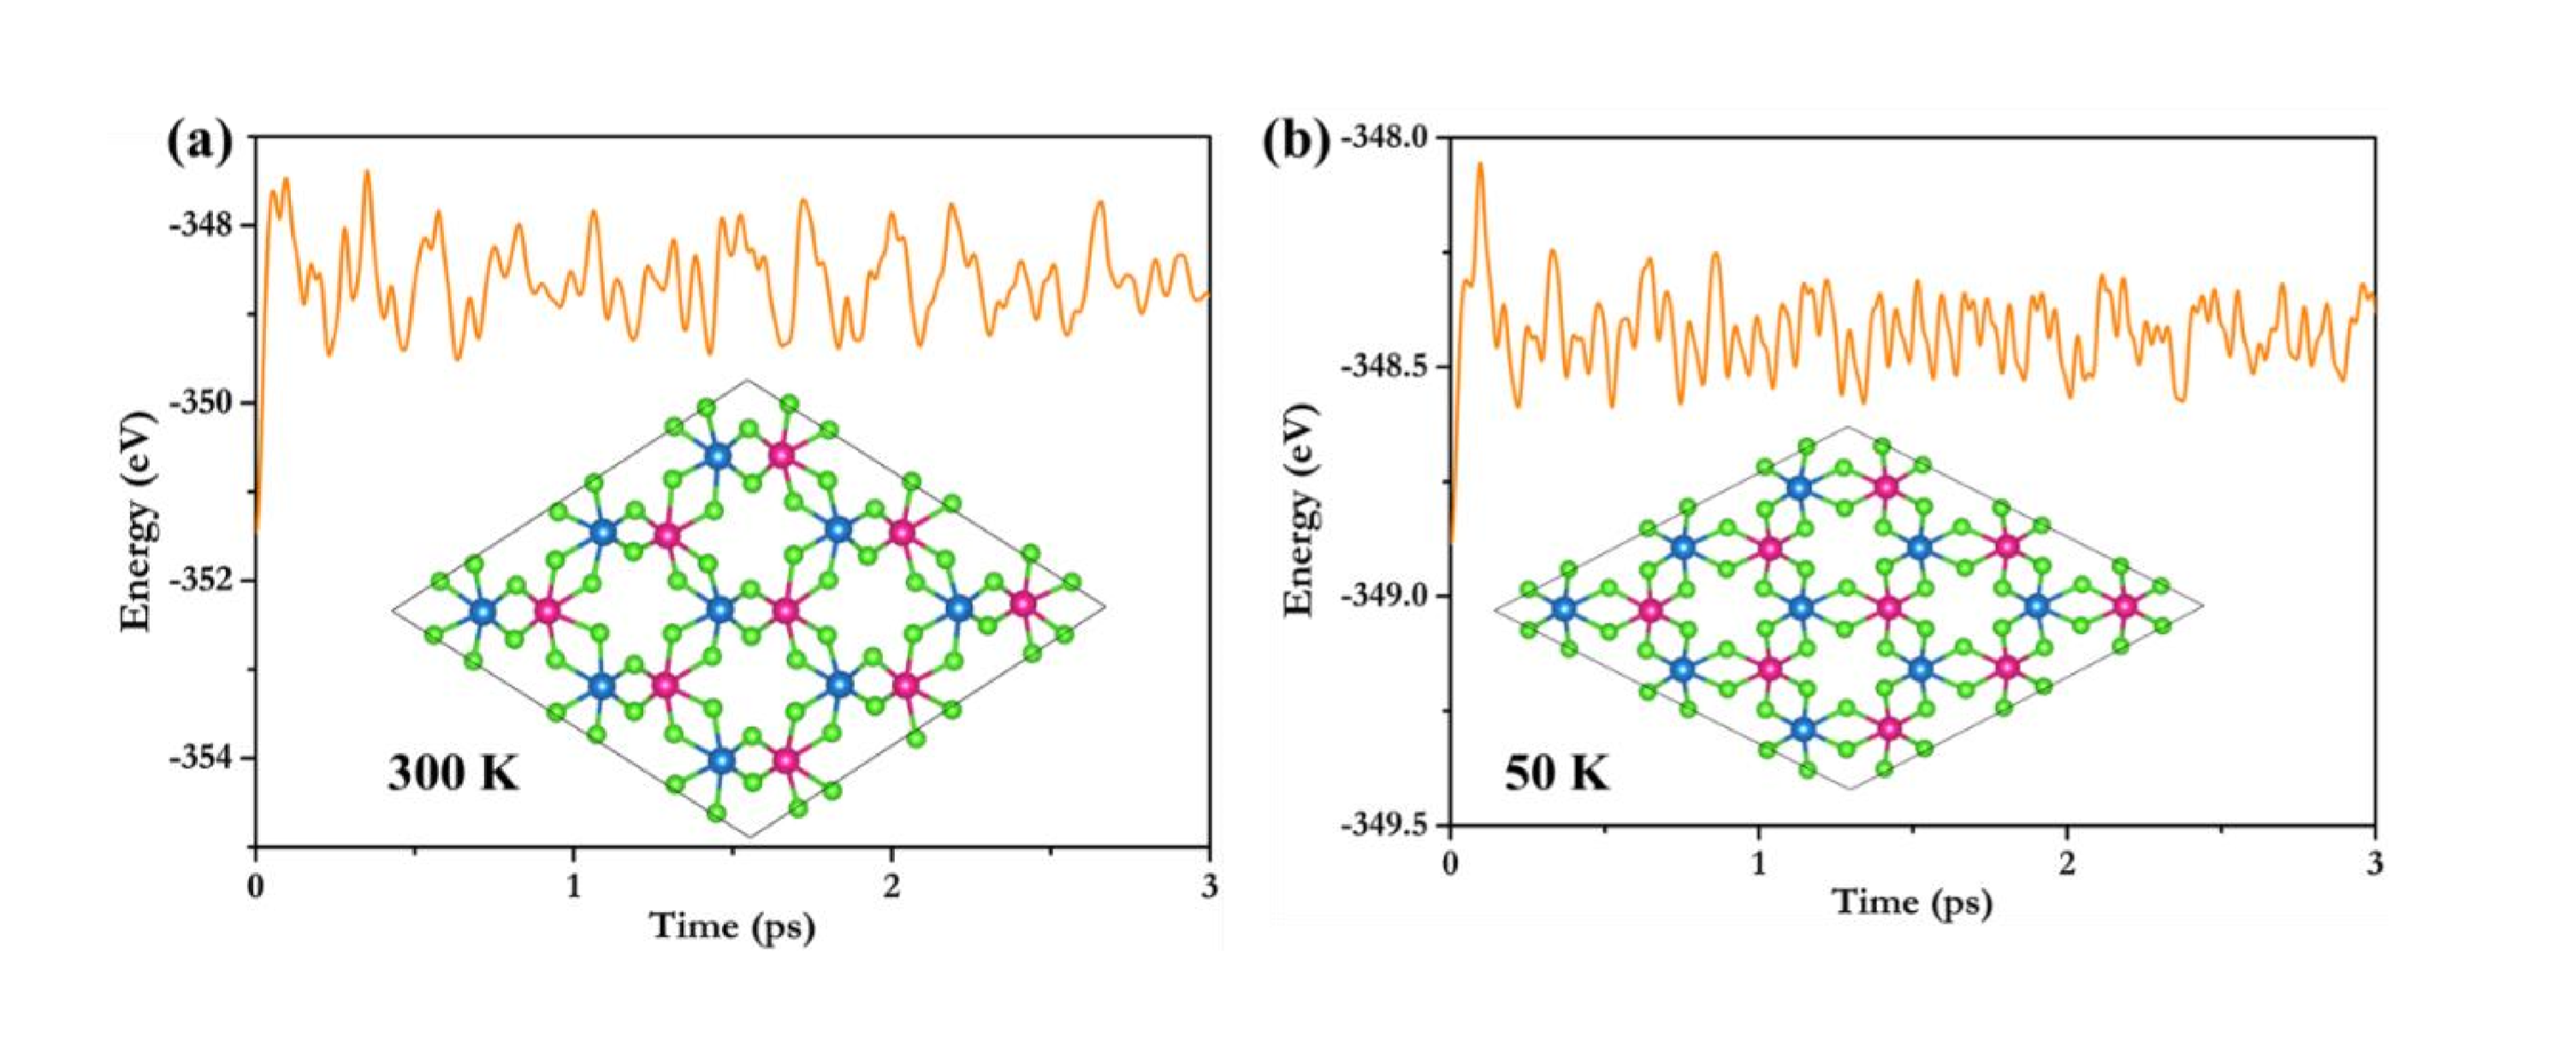
\includegraphics[width=0.8\textwidth]{./pic/020.png}
\caption{基于牛顿力学的分子动力学模拟\ 通过对D型与C型AIMD模拟,观察其总能量的波动。结果表明,D型结构在300K与C型在50K下是稳定的,在超过100K的情况下,C型总会自发向D型转变}

\label{dog020}
\end{figure}

通过第一性原理计算,$D_{3}-ReWCl_{6}$是没有带隙的导体,而两种具有铁电性的D型与C型则是具有0.67eV、0.38eV的半导体。而整个系统中的自旋轨道耦合几乎不会影响电子结构。\cite{ISI:A1993KJ51800070}

\begin{figure}[h]
    \centering
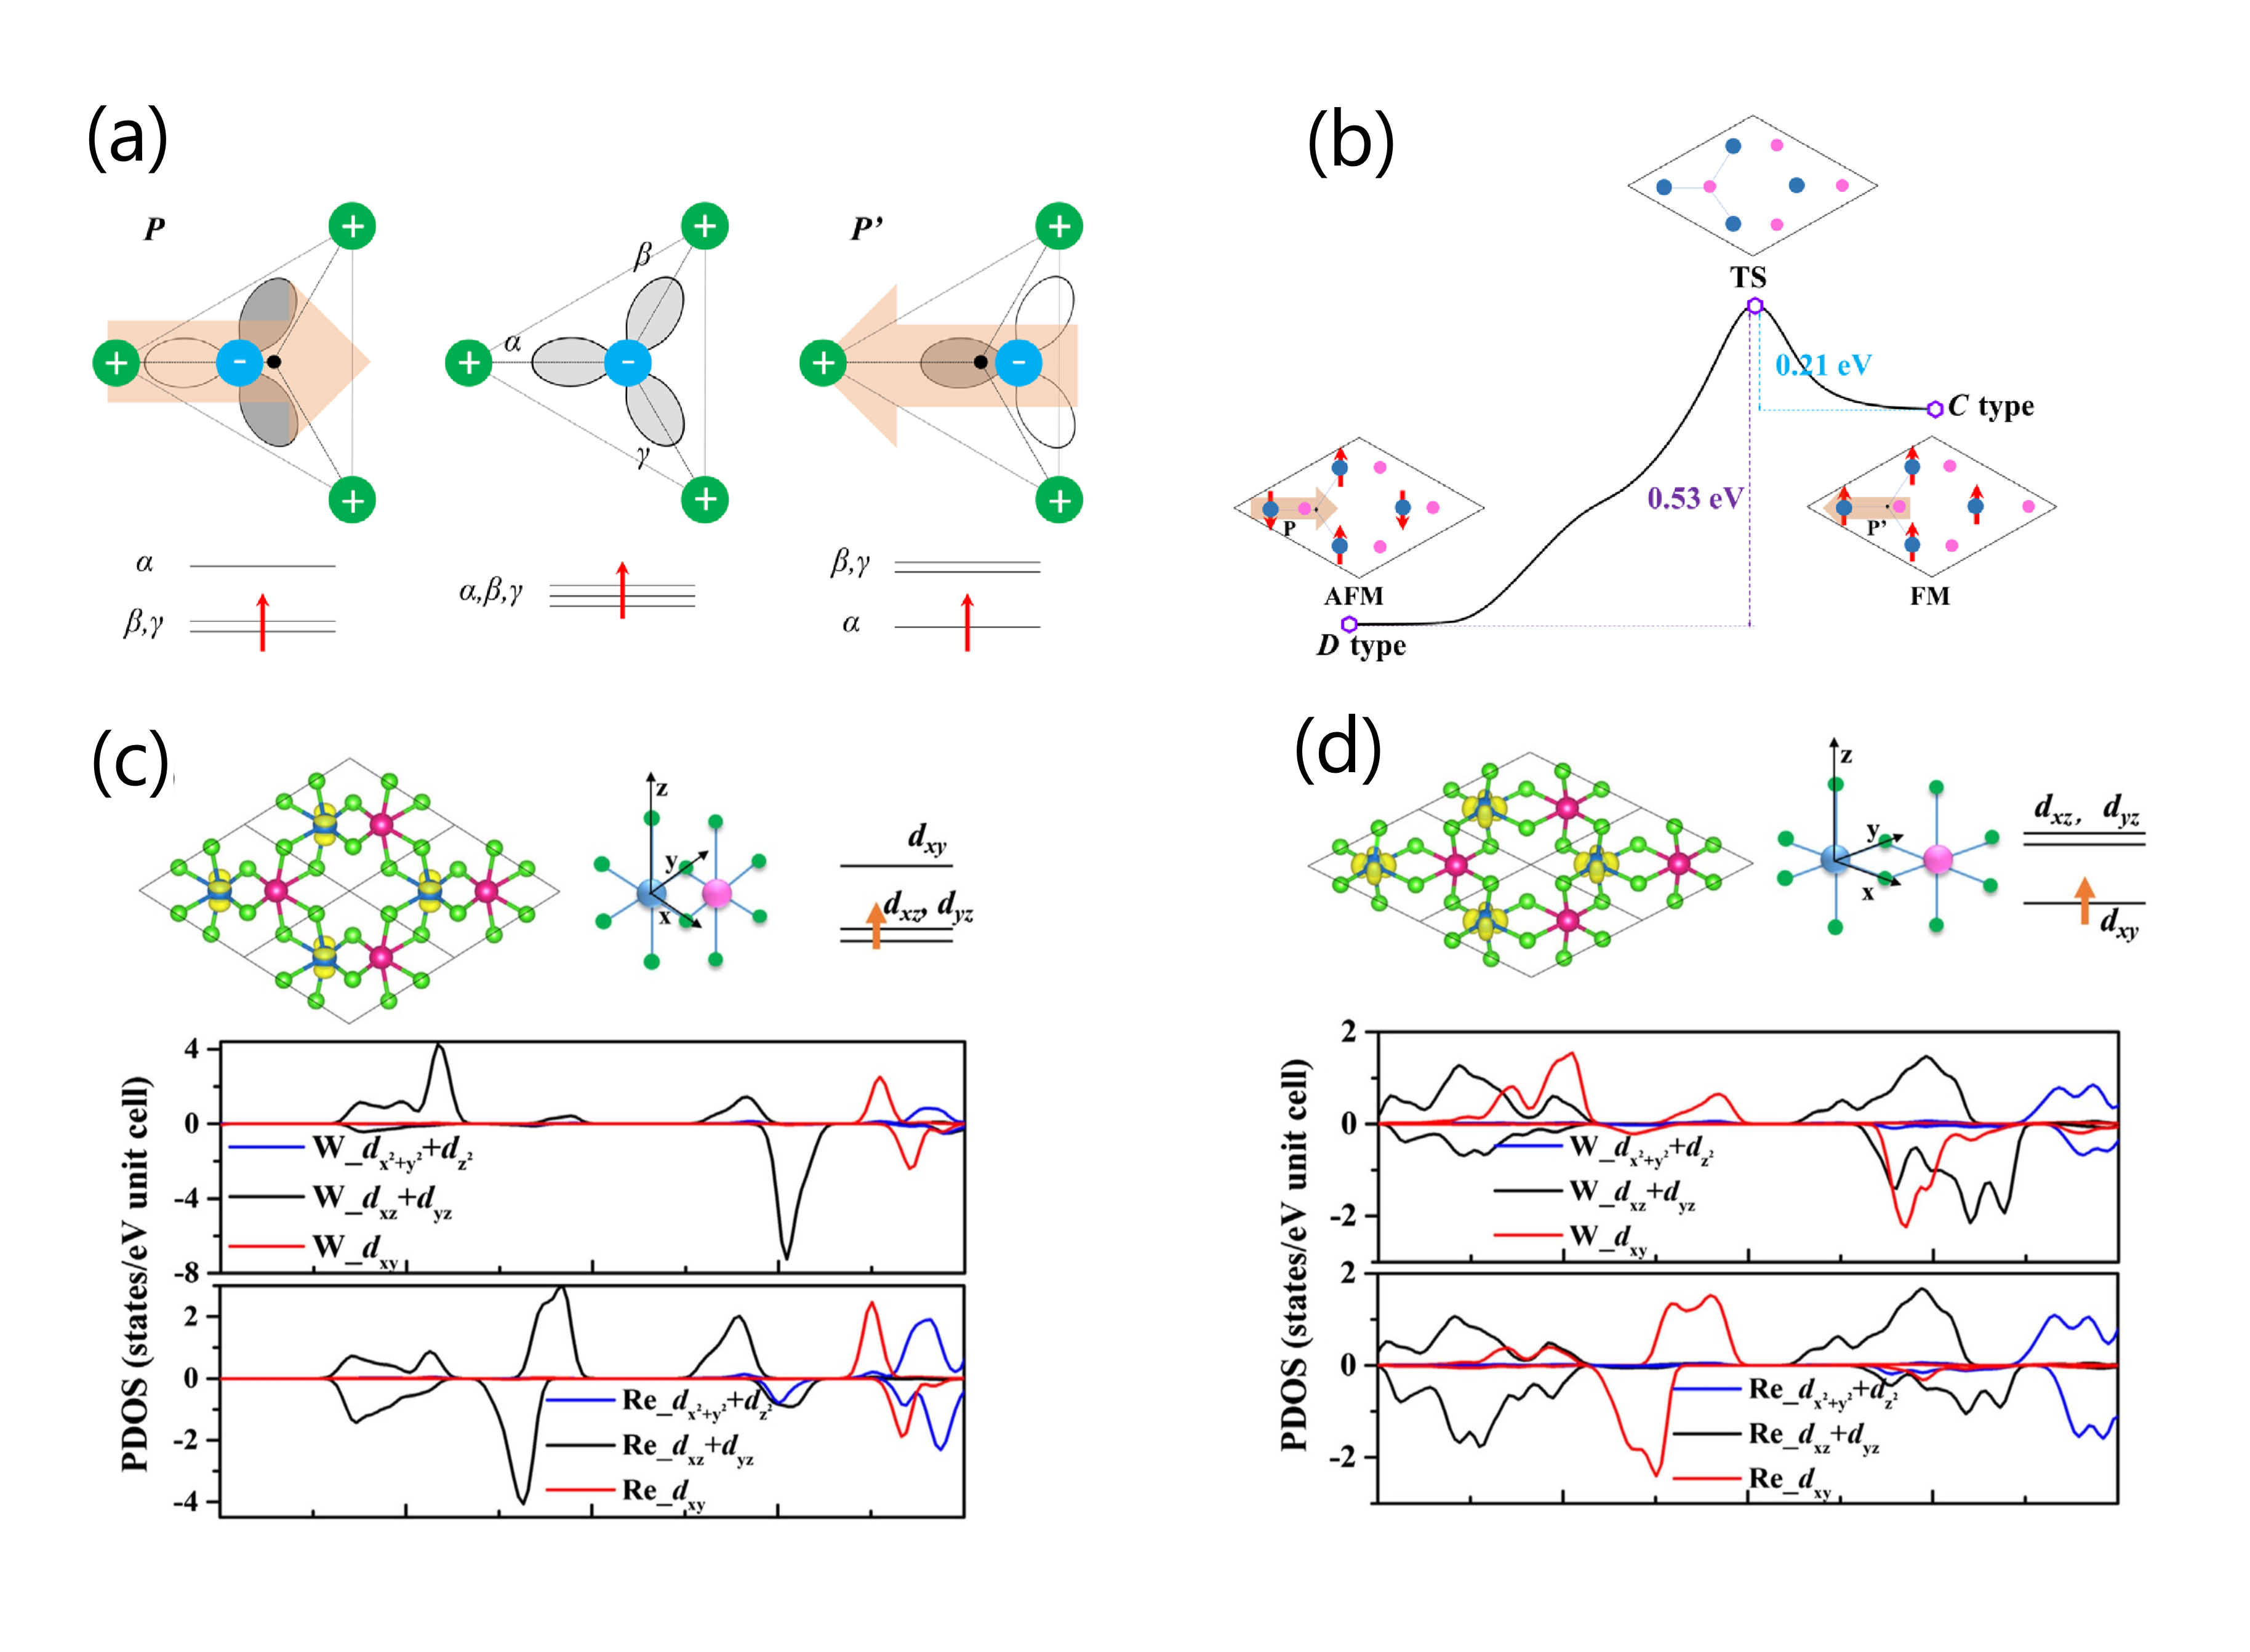
\includegraphics[width=0.8\textwidth]{./pic/022.png}
\caption{(a)$ReWCl_{6}$的D型、C型和高对称性$C_{3}$型的示意图\ 图中绿色与蓝色分别代表带电的正负离子,从图中可以看到高对称性$C_{3}$型仍然存在中心对称轴,在面内没有自发极化,相应的,电子能级结构也没有出现不对称的分离与能量变化,D型、C型结构中心金属阳离子发生了位置偏移,导致中心对称性消失,D型、C型两种铁电相位于三角形中心的阳离子偏移方向不同,所导致的这两种类型的自发极化方向相反,同样的,金属阳离子周边的电子运动所受到阴离子影响也会发生变化,这导致了D型、C型电子能级发生分裂与变化。(b)D型、C型两种铁电相之间的相变过程的动力学路径。蓝色代表W原子,红色代表Re原子,Cl原子被忽略,上下箭头代表自旋方向。在D型、C型两种铁电相之间有一个转化中间态势垒,D型的能量要高于C型,在发生两种铁电相变时,不仅仅自发极化方向会反转,系统的磁性质也会从反铁磁性与铁磁性之间转化。(c)(d)D型、C型两种的电子自旋态密度,两种不同类型$W_{t2g}$轨道不同占据情况。}

\label{dog022}
\end{figure}

受制于晶体的三角形结构,面内的电极化方向是收到限制的,两种铁电相D型和C型的电极化方向可以进行间隔120°的旋转,如果进行180°的反转,即进行电极化的反转,只能通过C型和D型之间的相变或者进行对整个结构的60°旋转。这一点可以通过在面内加入静电场来确认。与传统的二维铁电材料不同,二维$ReWCl_{6}$在发生电极化方向的反转时,会经历一个D型、C型之间的相变,在这种情形下,在自发极化方向反转的时候,电极化的变化不是连续的,中间有一个突变的过程,这种突变过程比正常的量子极化效应要大的多,突变来自于D型和C型,高自旋和低自旋状态之间的相变。\cite{WANG20122063}

\subsection{铁磁性}

根据Re元素和W的化合价,系统的铁磁性来源于$W^{5+}-d^{1}$的一个未成对电子贡献出的1$\mu_{B}$磁矩。而$Re^{+}-d^{6}$电子完全占据了$Re-t_{2g}$轨道,通过应用MLWFs方法对电子轨道能量进行分析,D型结构与C型结构自旋极化的电子结构不同。在C型中,由于$d_{xz}\text{和}d_{yz}$能量比较高,自旋磁矩电子主要占据$d_{xy}$轨道,在C型结构中自旋磁矩电子占据在$d_{xz}\text{和}d_{yz}$轨道。自旋哈密顿量可以写成:
\begin{equation}
    \hat{H}=-\sum_{i}(2J_{1}\vec{S}_{i}\cdot \vec{S}_{i,1}+ J_{2}\vec{S}_{i}\cdot \vec{S}_{i,2})
    \label{zixuan}
\end{equation}
其中$J_{1}\text{和}J_{2}$分别是在[1\ 0\ 0][0\ 1\ 0]方向和[1\ 1\ 0]方向上的交换积分。通过计算可得D型的$J_{1}\text{和}J_{2}$分别是2.00meV和−1.00meV,正负号表示反铁磁耦合与铁磁耦合,D型的基态是反铁磁性的。C型的$J_{1}\text{和}J_{2}$分别是-1.75meV和0.75meV ,基态是铁磁性的。\cite{PhysRevB.82.094116} 这个结果可以这样理解,反铁磁性的5d轨道交换积分与W之间的距离有关,短的W-W间距会增强反铁磁性,长的W-W距离会增强铁磁性,两种类行不同的W-W距离导致了铁磁性与反铁磁性的不同。蒙特卡洛模拟显示D型和C型的磁性临界温度在21K和10K左右。\cite{katsura2005spin}

\begin{figure}[h]
    \centering
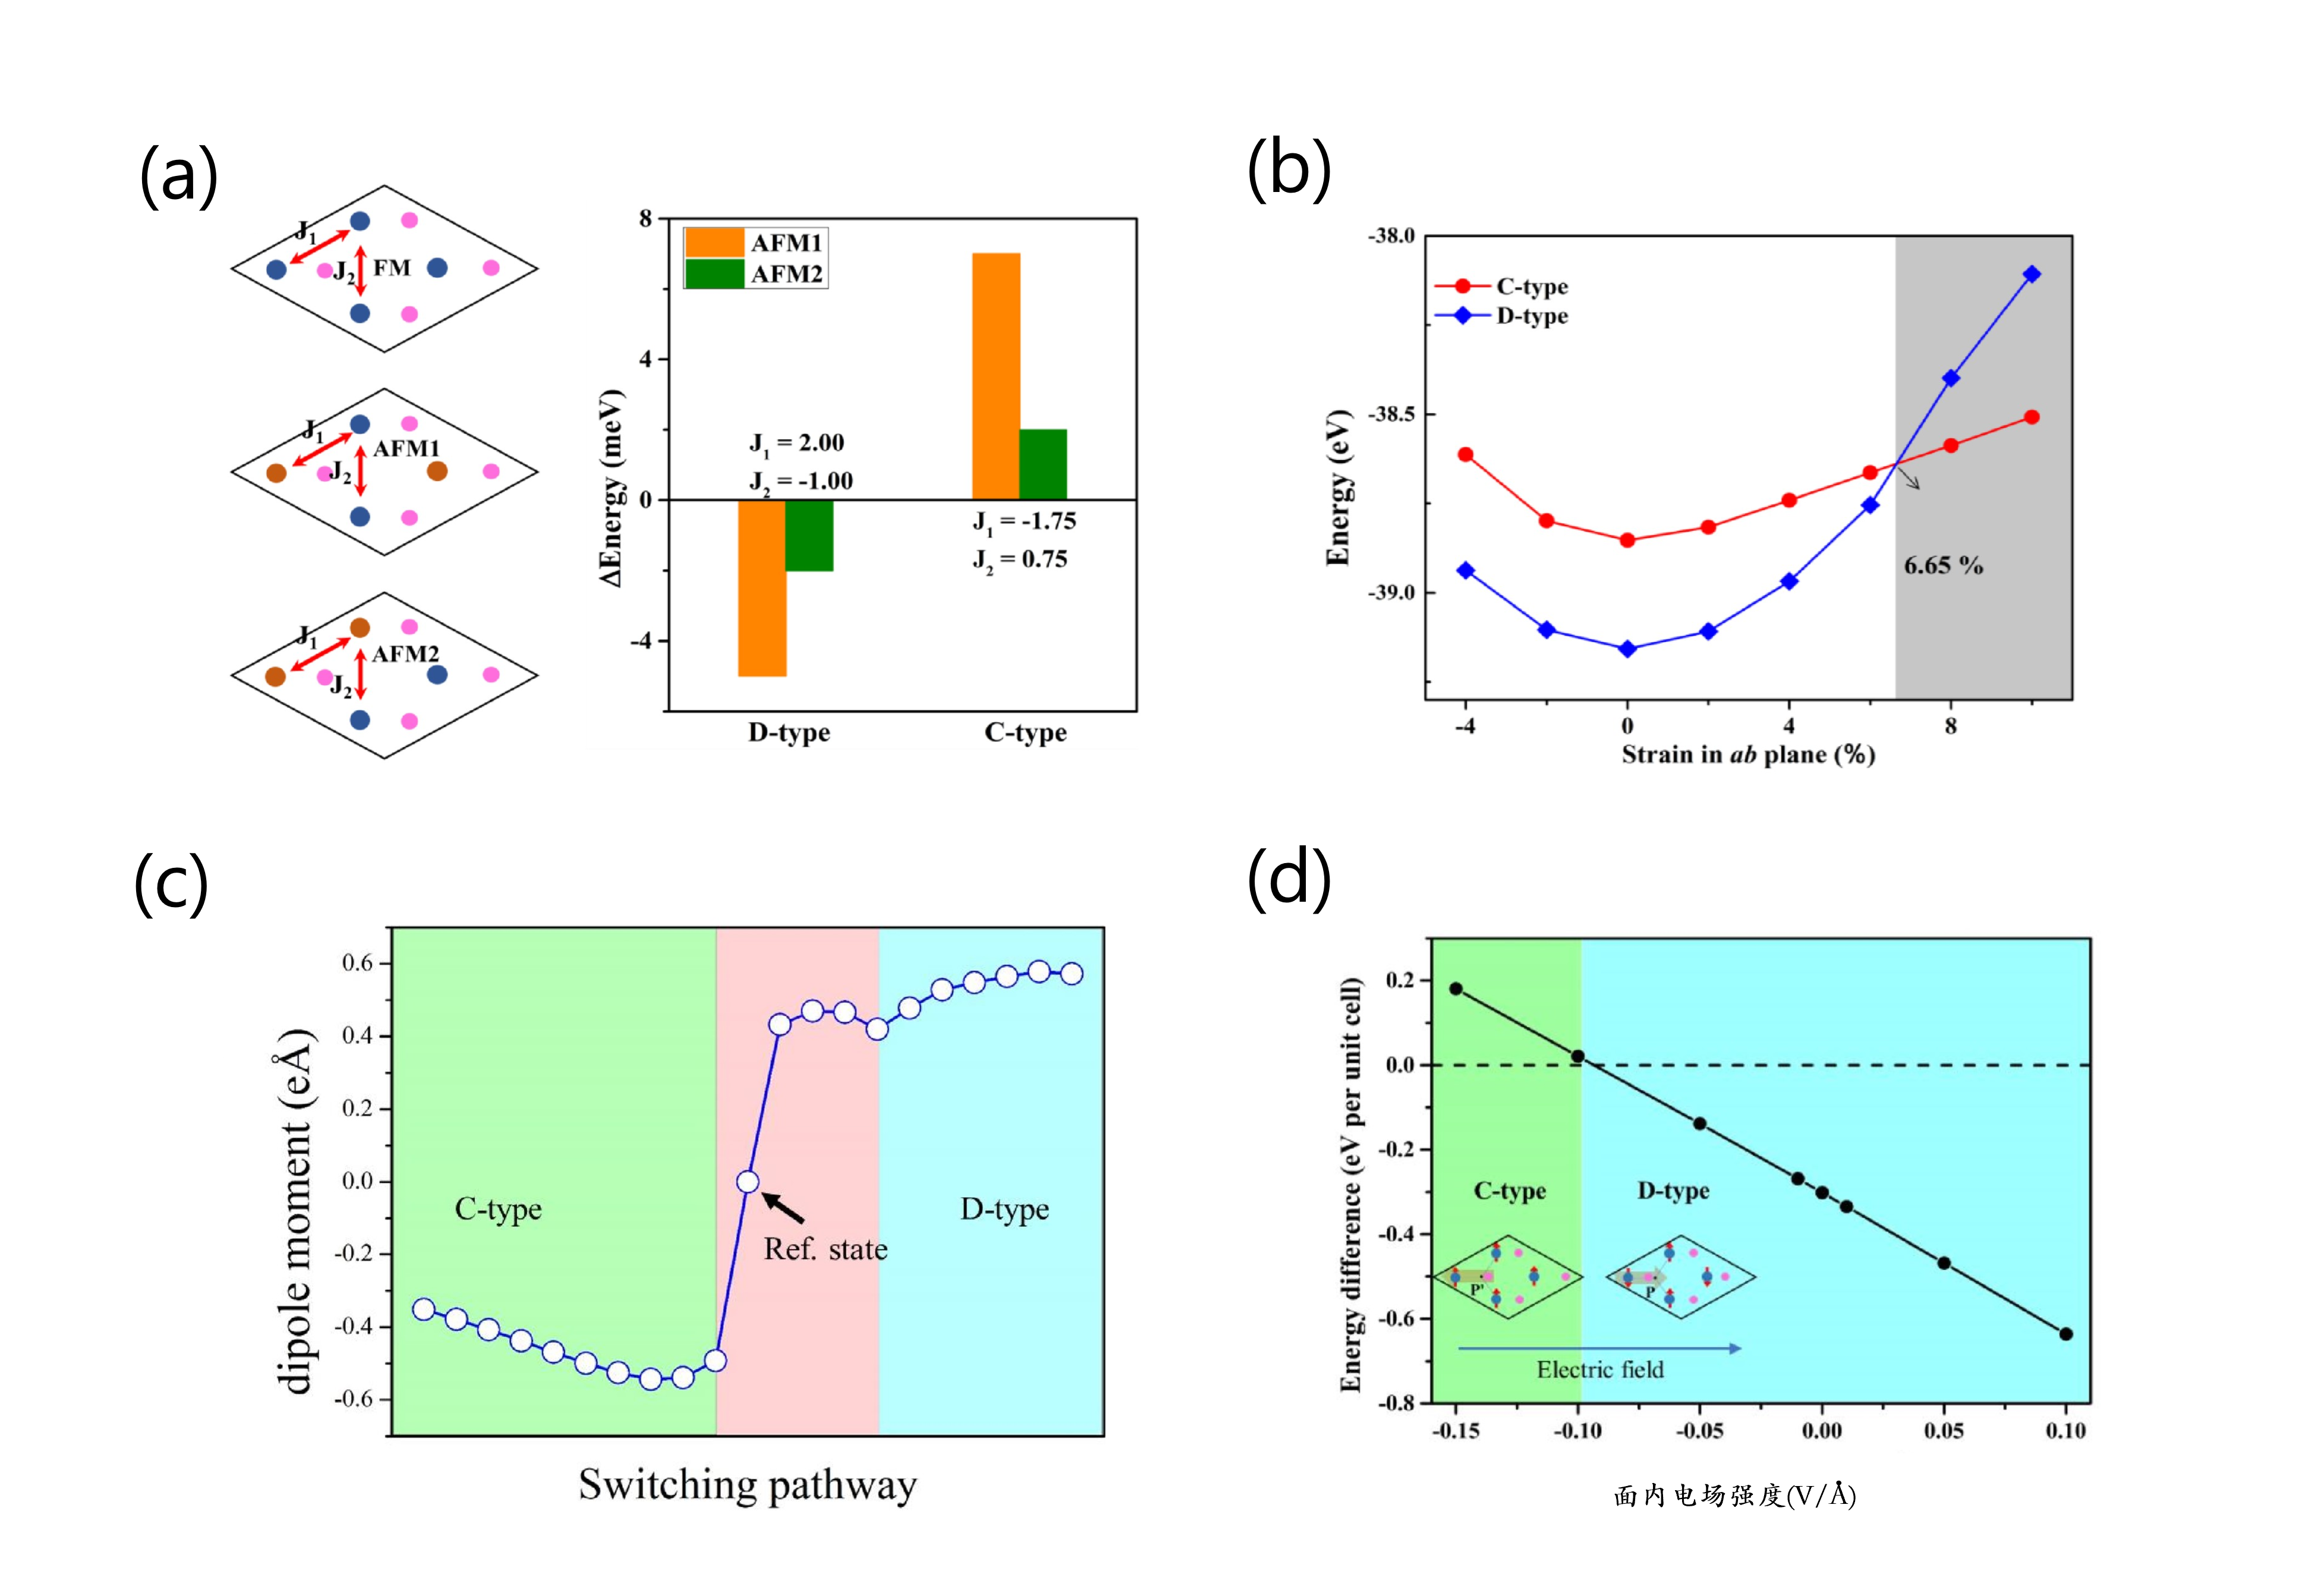
\includegraphics[width=0.8\textwidth]{./pic/023.png}
\caption{(a)$ReWCl_{6}$可能的几种磁矩排布方式,由两种反铁磁相和一种铁磁相,大实心圆表示W原子,小实心圆表示Re原子,深蓝色和橙色分别是向上自旋和下自旋状态,$J_{1}\text{和}J_{2}$分别是在[1\ 0\ 0][0\ 1\ 0]方向和[1\ 1\ 0]方向上的交换积分。右边是不同磁矩排布方式在不同类型下的交换积分和总能量,正负号表示反铁磁耦合与铁磁耦合,反铁磁的D型AFM1状态的能量最低。(b)双轴应变对D型与C型两种类型总能量的影响,在没有应变时D型的能量更低,在应变大于6.65\%时,C型的能量更低。\cite{ISI:000480497100035} 这表明在适当应变的条件下,也可以实现D型与C型两种类型的转换。(c)D型与C型之间转换时电偶极矩的变化。与一般铁电材料电极化的连续变化不同,$ReWCl_{6}$电极化方向反转时存在着一个突变过程,涉及到D型与C型之间的相变,转化中间存在着一个类似高对称性$C_{3}$型的没有电极化的状态。(d)在施加面内电场时D型与C型能量差的变化,电场的正负号分别表示沿[1\ -1\ 0]和[-1\ 1\ 0]方向的电场。沿[-1\ 1\ 0]方向足够大的面内电场可能会导致从D型过渡到C型,从而导致电极化的反转。}

\label{dog023}
\end{figure}

\subsection{电磁耦合}

作为一种第一类的二维多铁材料,通过常规的通常的电磁耦合方式的作用是微弱的,然而$ReWCl_{6}$的D型与C型两种状态电极化方向相反,铁磁性也不同,这在另一种层面上实现的电磁耦合。经过计算,$ReWCl_{6}$的电磁耦合强度可以达到$Fe/BaTiO_{3}$的水平。D型与C型两种状态的能带带隙也不同,D型与C型两种状态可以用外加电场的方式进行转化,这同样可以意味着可以通过外加电场调控电子结构。与常规的多铁材料的电磁耦合中磁化强度会随着外加电场变化不同,当施加的电场大于矫顽场时,极化方向会反转,磁相会同时改变,$ReWCl_{6}$的磁场强度并不会随着外加电场的增大而增大,因为在完成铁磁相与反铁磁相的切换之后没有明显的机制支持铁电性与铁磁性的强耦合。一般的多铁材料电磁耦合系数$\alpha=\mu_{0}|\Delta\bm{M}|/E$,但在$ReWCl_{6}$情况下这样的表述形式需要进行重新解释以适应$ReWCl_{6}$独特的电磁耦合方式。如果用铁磁相与反铁磁相转化时的$\Delta\bm{M}\text{和}E$,$\Delta\bm{M}$为改变极化方向前后的磁化强度变化,E为矫顽电场,进行计算,可以得出~666G(原文如此)的结果,比$Fe/BaTiO_{3}$的~120G大得多。

作为与铁电性关系更加密切的铁弹性,对二维$ReWCl_{6}$,在平面内部施加合适的应变也会导致D型与C型两种状态相互转化。\cite{ISI:000274700900024}



总的来说,$ReWCl_{6}$是一种新型的二维多铁材料。$ReWCl_{6}$通过一种特殊的铁电相与晶格结构耦合,进一步影响铁磁性的方式实现了铁电性铁磁性不同源的第一类多铁材料的强铁电铁磁耦合。通过施加合适的外电场实现面内电极化的反转与铁磁相与反铁磁相的转化,这些发现揭示了二维多铁性材料中磁相变电学控制的磁电耦合新机理,这很可能引起自旋电子学的研究和应用。从另一方面,$ReWCl_{6}$多铁性与电磁耦合产生的机制并不能支持通过磁场控制电极化或者是进行不同的铁磁性之间的转化,从这个角度看来,$ReWCl_{6}$的多铁性是不全面的,在将来的应用方面也许会受到一定的限制。